\documentclass[11pt]{article}

    \usepackage[breakable]{tcolorbox}
    \usepackage{parskip} % Stop auto-indenting (to mimic markdown behaviour)
    
    \usepackage{iftex}
    \ifPDFTeX
    	\usepackage[T1]{fontenc}
    	\usepackage{mathpazo}
    \else
    	\usepackage{fontspec}
    \fi

    % Basic figure setup, for now with no caption control since it's done
    % automatically by Pandoc (which extracts ![](path) syntax from Markdown).
    \usepackage{graphicx}
    % Maintain compatibility with old templates. Remove in nbconvert 6.0
    \let\Oldincludegraphics\includegraphics
    % Ensure that by default, figures have no caption (until we provide a
    % proper Figure object with a Caption API and a way to capture that
    % in the conversion process - todo).
    \usepackage{caption}
%     \DeclareCaptionFormat{nocaption}{}
%     \captionsetup{format=nocaption,aboveskip=0pt,belowskip=0pt}

    \usepackage{float}
    \floatplacement{figure}{H} % forces figures to be placed at the correct location
    \usepackage{xcolor} % Allow colors to be defined
    \usepackage{enumerate} % Needed for markdown enumerations to work
    \usepackage{geometry} % Used to adjust the document margins
    \usepackage{amsmath} % Equations
    \usepackage{amssymb} % Equations
    \usepackage{textcomp} % defines textquotesingle
    % Hack from http://tex.stackexchange.com/a/47451/13684:
    \AtBeginDocument{%
        \def\PYZsq{\textquotesingle}% Upright quotes in Pygmentized code
    }
    \usepackage{upquote} % Upright quotes for verbatim code
    \usepackage{eurosym} % defines \euro
    \usepackage[mathletters]{ucs} % Extended unicode (utf-8) support
    \usepackage{fancyvrb} % verbatim replacement that allows latex
    \usepackage{grffile} % extends the file name processing of package graphics 
                         % to support a larger range
    \makeatletter % fix for old versions of grffile with XeLaTeX
    \@ifpackagelater{grffile}{2019/11/01}
    {
      % Do nothing on new versions
    }
    {
      \def\Gread@@xetex#1{%
        \IfFileExists{"\Gin@base".bb}%
        {\Gread@eps{\Gin@base.bb}}%
        {\Gread@@xetex@aux#1}%
      }
    }
    \makeatother
    \usepackage[Export]{adjustbox} % Used to constrain images to a maximum size
    \adjustboxset{max size={0.9\linewidth}{0.9\paperheight}}

    % The hyperref package gives us a pdf with properly built
    % internal navigation ('pdf bookmarks' for the table of contents,
    % internal cross-reference links, web links for URLs, etc.)
    \usepackage{hyperref}
    % The default LaTeX title has an obnoxious amount of whitespace. By default,
    % titling removes some of it. It also provides customization options.
    \usepackage{titling}
    \usepackage{longtable} % longtable support required by pandoc >1.10
    \usepackage{booktabs}  % table support for pandoc > 1.12.2
    \usepackage[inline]{enumitem} % IRkernel/repr support (it uses the enumerate* environment)
    \usepackage[normalem]{ulem} % ulem is needed to support strikethroughs (\sout)
                                % normalem makes italics be italics, not underlines
    \usepackage{mathrsfs}
    

    
    % Colors for the hyperref package
    \definecolor{urlcolor}{rgb}{0,.145,.698}
    \definecolor{linkcolor}{rgb}{.71,0.21,0.01}
    \definecolor{citecolor}{rgb}{.12,.54,.11}

    % ANSI colors
    \definecolor{ansi-black}{HTML}{3E424D}
    \definecolor{ansi-black-intense}{HTML}{282C36}
    \definecolor{ansi-red}{HTML}{E75C58}
    \definecolor{ansi-red-intense}{HTML}{B22B31}
    \definecolor{ansi-green}{HTML}{00A250}
    \definecolor{ansi-green-intense}{HTML}{007427}
    \definecolor{ansi-yellow}{HTML}{DDB62B}
    \definecolor{ansi-yellow-intense}{HTML}{B27D12}
    \definecolor{ansi-blue}{HTML}{208FFB}
    \definecolor{ansi-blue-intense}{HTML}{0065CA}
    \definecolor{ansi-magenta}{HTML}{D160C4}
    \definecolor{ansi-magenta-intense}{HTML}{A03196}
    \definecolor{ansi-cyan}{HTML}{60C6C8}
    \definecolor{ansi-cyan-intense}{HTML}{258F8F}
    \definecolor{ansi-white}{HTML}{C5C1B4}
    \definecolor{ansi-white-intense}{HTML}{A1A6B2}
    \definecolor{ansi-default-inverse-fg}{HTML}{FFFFFF}
    \definecolor{ansi-default-inverse-bg}{HTML}{000000}

    % common color for the border for error outputs.
    \definecolor{outerrorbackground}{HTML}{FFDFDF}

    % commands and environments needed by pandoc snippets
    % extracted from the output of `pandoc -s`
    \providecommand{\tightlist}{%
      \setlength{\itemsep}{0pt}\setlength{\parskip}{0pt}}
    \DefineVerbatimEnvironment{Highlighting}{Verbatim}{commandchars=\\\{\}}
    % Add ',fontsize=\small' for more characters per line
    \newenvironment{Shaded}{}{}
    \newcommand{\KeywordTok}[1]{\textcolor[rgb]{0.00,0.44,0.13}{\textbf{{#1}}}}
    \newcommand{\DataTypeTok}[1]{\textcolor[rgb]{0.56,0.13,0.00}{{#1}}}
    \newcommand{\DecValTok}[1]{\textcolor[rgb]{0.25,0.63,0.44}{{#1}}}
    \newcommand{\BaseNTok}[1]{\textcolor[rgb]{0.25,0.63,0.44}{{#1}}}
    \newcommand{\FloatTok}[1]{\textcolor[rgb]{0.25,0.63,0.44}{{#1}}}
    \newcommand{\CharTok}[1]{\textcolor[rgb]{0.25,0.44,0.63}{{#1}}}
    \newcommand{\StringTok}[1]{\textcolor[rgb]{0.25,0.44,0.63}{{#1}}}
    \newcommand{\CommentTok}[1]{\textcolor[rgb]{0.38,0.63,0.69}{\textit{{#1}}}}
    \newcommand{\OtherTok}[1]{\textcolor[rgb]{0.00,0.44,0.13}{{#1}}}
    \newcommand{\AlertTok}[1]{\textcolor[rgb]{1.00,0.00,0.00}{\textbf{{#1}}}}
    \newcommand{\FunctionTok}[1]{\textcolor[rgb]{0.02,0.16,0.49}{{#1}}}
    \newcommand{\RegionMarkerTok}[1]{{#1}}
    \newcommand{\ErrorTok}[1]{\textcolor[rgb]{1.00,0.00,0.00}{\textbf{{#1}}}}
    \newcommand{\NormalTok}[1]{{#1}}
    
    % Additional commands for more recent versions of Pandoc
    \newcommand{\ConstantTok}[1]{\textcolor[rgb]{0.53,0.00,0.00}{{#1}}}
    \newcommand{\SpecialCharTok}[1]{\textcolor[rgb]{0.25,0.44,0.63}{{#1}}}
    \newcommand{\VerbatimStringTok}[1]{\textcolor[rgb]{0.25,0.44,0.63}{{#1}}}
    \newcommand{\SpecialStringTok}[1]{\textcolor[rgb]{0.73,0.40,0.53}{{#1}}}
    \newcommand{\ImportTok}[1]{{#1}}
    \newcommand{\DocumentationTok}[1]{\textcolor[rgb]{0.73,0.13,0.13}{\textit{{#1}}}}
    \newcommand{\AnnotationTok}[1]{\textcolor[rgb]{0.38,0.63,0.69}{\textbf{\textit{{#1}}}}}
    \newcommand{\CommentVarTok}[1]{\textcolor[rgb]{0.38,0.63,0.69}{\textbf{\textit{{#1}}}}}
    \newcommand{\VariableTok}[1]{\textcolor[rgb]{0.10,0.09,0.49}{{#1}}}
    \newcommand{\ControlFlowTok}[1]{\textcolor[rgb]{0.00,0.44,0.13}{\textbf{{#1}}}}
    \newcommand{\OperatorTok}[1]{\textcolor[rgb]{0.40,0.40,0.40}{{#1}}}
    \newcommand{\BuiltInTok}[1]{{#1}}
    \newcommand{\ExtensionTok}[1]{{#1}}
    \newcommand{\PreprocessorTok}[1]{\textcolor[rgb]{0.74,0.48,0.00}{{#1}}}
    \newcommand{\AttributeTok}[1]{\textcolor[rgb]{0.49,0.56,0.16}{{#1}}}
    \newcommand{\InformationTok}[1]{\textcolor[rgb]{0.38,0.63,0.69}{\textbf{\textit{{#1}}}}}
    \newcommand{\WarningTok}[1]{\textcolor[rgb]{0.38,0.63,0.69}{\textbf{\textit{{#1}}}}}
    
    
    % Define a nice break command that doesn't care if a line doesn't already
    % exist.
    \def\br{\hspace*{\fill} \\* }
    % Math Jax compatibility definitions
    \def\gt{>}
    \def\lt{<}
    \let\Oldtex\TeX
    \let\Oldlatex\LaTeX
    \renewcommand{\TeX}{\textrm{\Oldtex}}
    \renewcommand{\LaTeX}{\textrm{\Oldlatex}}
    % Document parameters
    % Document title
    \title{Remarks on COVID-19 Dynamics in Switzerland}
    \author{Flávio Codeço Coelho}
    
    
    
    
    
% Pygments definitions
\makeatletter
\def\PY@reset{\let\PY@it=\relax \let\PY@bf=\relax%
    \let\PY@ul=\relax \let\PY@tc=\relax%
    \let\PY@bc=\relax \let\PY@ff=\relax}
\def\PY@tok#1{\csname PY@tok@#1\endcsname}
\def\PY@toks#1+{\ifx\relax#1\empty\else%
    \PY@tok{#1}\expandafter\PY@toks\fi}
\def\PY@do#1{\PY@bc{\PY@tc{\PY@ul{%
    \PY@it{\PY@bf{\PY@ff{#1}}}}}}}
\def\PY#1#2{\PY@reset\PY@toks#1+\relax+\PY@do{#2}}

\expandafter\def\csname PY@tok@w\endcsname{\def\PY@tc##1{\textcolor[rgb]{0.73,0.73,0.73}{##1}}}
\expandafter\def\csname PY@tok@c\endcsname{\let\PY@it=\textit\def\PY@tc##1{\textcolor[rgb]{0.25,0.50,0.50}{##1}}}
\expandafter\def\csname PY@tok@cp\endcsname{\def\PY@tc##1{\textcolor[rgb]{0.74,0.48,0.00}{##1}}}
\expandafter\def\csname PY@tok@k\endcsname{\let\PY@bf=\textbf\def\PY@tc##1{\textcolor[rgb]{0.00,0.50,0.00}{##1}}}
\expandafter\def\csname PY@tok@kp\endcsname{\def\PY@tc##1{\textcolor[rgb]{0.00,0.50,0.00}{##1}}}
\expandafter\def\csname PY@tok@kt\endcsname{\def\PY@tc##1{\textcolor[rgb]{0.69,0.00,0.25}{##1}}}
\expandafter\def\csname PY@tok@o\endcsname{\def\PY@tc##1{\textcolor[rgb]{0.40,0.40,0.40}{##1}}}
\expandafter\def\csname PY@tok@ow\endcsname{\let\PY@bf=\textbf\def\PY@tc##1{\textcolor[rgb]{0.67,0.13,1.00}{##1}}}
\expandafter\def\csname PY@tok@nb\endcsname{\def\PY@tc##1{\textcolor[rgb]{0.00,0.50,0.00}{##1}}}
\expandafter\def\csname PY@tok@nf\endcsname{\def\PY@tc##1{\textcolor[rgb]{0.00,0.00,1.00}{##1}}}
\expandafter\def\csname PY@tok@nc\endcsname{\let\PY@bf=\textbf\def\PY@tc##1{\textcolor[rgb]{0.00,0.00,1.00}{##1}}}
\expandafter\def\csname PY@tok@nn\endcsname{\let\PY@bf=\textbf\def\PY@tc##1{\textcolor[rgb]{0.00,0.00,1.00}{##1}}}
\expandafter\def\csname PY@tok@ne\endcsname{\let\PY@bf=\textbf\def\PY@tc##1{\textcolor[rgb]{0.82,0.25,0.23}{##1}}}
\expandafter\def\csname PY@tok@nv\endcsname{\def\PY@tc##1{\textcolor[rgb]{0.10,0.09,0.49}{##1}}}
\expandafter\def\csname PY@tok@no\endcsname{\def\PY@tc##1{\textcolor[rgb]{0.53,0.00,0.00}{##1}}}
\expandafter\def\csname PY@tok@nl\endcsname{\def\PY@tc##1{\textcolor[rgb]{0.63,0.63,0.00}{##1}}}
\expandafter\def\csname PY@tok@ni\endcsname{\let\PY@bf=\textbf\def\PY@tc##1{\textcolor[rgb]{0.60,0.60,0.60}{##1}}}
\expandafter\def\csname PY@tok@na\endcsname{\def\PY@tc##1{\textcolor[rgb]{0.49,0.56,0.16}{##1}}}
\expandafter\def\csname PY@tok@nt\endcsname{\let\PY@bf=\textbf\def\PY@tc##1{\textcolor[rgb]{0.00,0.50,0.00}{##1}}}
\expandafter\def\csname PY@tok@nd\endcsname{\def\PY@tc##1{\textcolor[rgb]{0.67,0.13,1.00}{##1}}}
\expandafter\def\csname PY@tok@s\endcsname{\def\PY@tc##1{\textcolor[rgb]{0.73,0.13,0.13}{##1}}}
\expandafter\def\csname PY@tok@sd\endcsname{\let\PY@it=\textit\def\PY@tc##1{\textcolor[rgb]{0.73,0.13,0.13}{##1}}}
\expandafter\def\csname PY@tok@si\endcsname{\let\PY@bf=\textbf\def\PY@tc##1{\textcolor[rgb]{0.73,0.40,0.53}{##1}}}
\expandafter\def\csname PY@tok@se\endcsname{\let\PY@bf=\textbf\def\PY@tc##1{\textcolor[rgb]{0.73,0.40,0.13}{##1}}}
\expandafter\def\csname PY@tok@sr\endcsname{\def\PY@tc##1{\textcolor[rgb]{0.73,0.40,0.53}{##1}}}
\expandafter\def\csname PY@tok@ss\endcsname{\def\PY@tc##1{\textcolor[rgb]{0.10,0.09,0.49}{##1}}}
\expandafter\def\csname PY@tok@sx\endcsname{\def\PY@tc##1{\textcolor[rgb]{0.00,0.50,0.00}{##1}}}
\expandafter\def\csname PY@tok@m\endcsname{\def\PY@tc##1{\textcolor[rgb]{0.40,0.40,0.40}{##1}}}
\expandafter\def\csname PY@tok@gh\endcsname{\let\PY@bf=\textbf\def\PY@tc##1{\textcolor[rgb]{0.00,0.00,0.50}{##1}}}
\expandafter\def\csname PY@tok@gu\endcsname{\let\PY@bf=\textbf\def\PY@tc##1{\textcolor[rgb]{0.50,0.00,0.50}{##1}}}
\expandafter\def\csname PY@tok@gd\endcsname{\def\PY@tc##1{\textcolor[rgb]{0.63,0.00,0.00}{##1}}}
\expandafter\def\csname PY@tok@gi\endcsname{\def\PY@tc##1{\textcolor[rgb]{0.00,0.63,0.00}{##1}}}
\expandafter\def\csname PY@tok@gr\endcsname{\def\PY@tc##1{\textcolor[rgb]{1.00,0.00,0.00}{##1}}}
\expandafter\def\csname PY@tok@ge\endcsname{\let\PY@it=\textit}
\expandafter\def\csname PY@tok@gs\endcsname{\let\PY@bf=\textbf}
\expandafter\def\csname PY@tok@gp\endcsname{\let\PY@bf=\textbf\def\PY@tc##1{\textcolor[rgb]{0.00,0.00,0.50}{##1}}}
\expandafter\def\csname PY@tok@go\endcsname{\def\PY@tc##1{\textcolor[rgb]{0.53,0.53,0.53}{##1}}}
\expandafter\def\csname PY@tok@gt\endcsname{\def\PY@tc##1{\textcolor[rgb]{0.00,0.27,0.87}{##1}}}
\expandafter\def\csname PY@tok@err\endcsname{\def\PY@bc##1{\setlength{\fboxsep}{0pt}\fcolorbox[rgb]{1.00,0.00,0.00}{1,1,1}{\strut ##1}}}
\expandafter\def\csname PY@tok@kc\endcsname{\let\PY@bf=\textbf\def\PY@tc##1{\textcolor[rgb]{0.00,0.50,0.00}{##1}}}
\expandafter\def\csname PY@tok@kd\endcsname{\let\PY@bf=\textbf\def\PY@tc##1{\textcolor[rgb]{0.00,0.50,0.00}{##1}}}
\expandafter\def\csname PY@tok@kn\endcsname{\let\PY@bf=\textbf\def\PY@tc##1{\textcolor[rgb]{0.00,0.50,0.00}{##1}}}
\expandafter\def\csname PY@tok@kr\endcsname{\let\PY@bf=\textbf\def\PY@tc##1{\textcolor[rgb]{0.00,0.50,0.00}{##1}}}
\expandafter\def\csname PY@tok@bp\endcsname{\def\PY@tc##1{\textcolor[rgb]{0.00,0.50,0.00}{##1}}}
\expandafter\def\csname PY@tok@fm\endcsname{\def\PY@tc##1{\textcolor[rgb]{0.00,0.00,1.00}{##1}}}
\expandafter\def\csname PY@tok@vc\endcsname{\def\PY@tc##1{\textcolor[rgb]{0.10,0.09,0.49}{##1}}}
\expandafter\def\csname PY@tok@vg\endcsname{\def\PY@tc##1{\textcolor[rgb]{0.10,0.09,0.49}{##1}}}
\expandafter\def\csname PY@tok@vi\endcsname{\def\PY@tc##1{\textcolor[rgb]{0.10,0.09,0.49}{##1}}}
\expandafter\def\csname PY@tok@vm\endcsname{\def\PY@tc##1{\textcolor[rgb]{0.10,0.09,0.49}{##1}}}
\expandafter\def\csname PY@tok@sa\endcsname{\def\PY@tc##1{\textcolor[rgb]{0.73,0.13,0.13}{##1}}}
\expandafter\def\csname PY@tok@sb\endcsname{\def\PY@tc##1{\textcolor[rgb]{0.73,0.13,0.13}{##1}}}
\expandafter\def\csname PY@tok@sc\endcsname{\def\PY@tc##1{\textcolor[rgb]{0.73,0.13,0.13}{##1}}}
\expandafter\def\csname PY@tok@dl\endcsname{\def\PY@tc##1{\textcolor[rgb]{0.73,0.13,0.13}{##1}}}
\expandafter\def\csname PY@tok@s2\endcsname{\def\PY@tc##1{\textcolor[rgb]{0.73,0.13,0.13}{##1}}}
\expandafter\def\csname PY@tok@sh\endcsname{\def\PY@tc##1{\textcolor[rgb]{0.73,0.13,0.13}{##1}}}
\expandafter\def\csname PY@tok@s1\endcsname{\def\PY@tc##1{\textcolor[rgb]{0.73,0.13,0.13}{##1}}}
\expandafter\def\csname PY@tok@mb\endcsname{\def\PY@tc##1{\textcolor[rgb]{0.40,0.40,0.40}{##1}}}
\expandafter\def\csname PY@tok@mf\endcsname{\def\PY@tc##1{\textcolor[rgb]{0.40,0.40,0.40}{##1}}}
\expandafter\def\csname PY@tok@mh\endcsname{\def\PY@tc##1{\textcolor[rgb]{0.40,0.40,0.40}{##1}}}
\expandafter\def\csname PY@tok@mi\endcsname{\def\PY@tc##1{\textcolor[rgb]{0.40,0.40,0.40}{##1}}}
\expandafter\def\csname PY@tok@il\endcsname{\def\PY@tc##1{\textcolor[rgb]{0.40,0.40,0.40}{##1}}}
\expandafter\def\csname PY@tok@mo\endcsname{\def\PY@tc##1{\textcolor[rgb]{0.40,0.40,0.40}{##1}}}
\expandafter\def\csname PY@tok@ch\endcsname{\let\PY@it=\textit\def\PY@tc##1{\textcolor[rgb]{0.25,0.50,0.50}{##1}}}
\expandafter\def\csname PY@tok@cm\endcsname{\let\PY@it=\textit\def\PY@tc##1{\textcolor[rgb]{0.25,0.50,0.50}{##1}}}
\expandafter\def\csname PY@tok@cpf\endcsname{\let\PY@it=\textit\def\PY@tc##1{\textcolor[rgb]{0.25,0.50,0.50}{##1}}}
\expandafter\def\csname PY@tok@c1\endcsname{\let\PY@it=\textit\def\PY@tc##1{\textcolor[rgb]{0.25,0.50,0.50}{##1}}}
\expandafter\def\csname PY@tok@cs\endcsname{\let\PY@it=\textit\def\PY@tc##1{\textcolor[rgb]{0.25,0.50,0.50}{##1}}}

\def\PYZbs{\char`\\}
\def\PYZus{\char`\_}
\def\PYZob{\char`\{}
\def\PYZcb{\char`\}}
\def\PYZca{\char`\^}
\def\PYZam{\char`\&}
\def\PYZlt{\char`\<}
\def\PYZgt{\char`\>}
\def\PYZsh{\char`\#}
\def\PYZpc{\char`\%}
\def\PYZdl{\char`\$}
\def\PYZhy{\char`\-}
\def\PYZsq{\char`\'}
\def\PYZdq{\char`\"}
\def\PYZti{\char`\~}
% for compatibility with earlier versions
\def\PYZat{@}
\def\PYZlb{[}
\def\PYZrb{]}
\makeatother


    % For linebreaks inside Verbatim environment from package fancyvrb. 
    \makeatletter
        \newbox\Wrappedcontinuationbox 
        \newbox\Wrappedvisiblespacebox 
        \newcommand*\Wrappedvisiblespace {\textcolor{red}{\textvisiblespace}} 
        \newcommand*\Wrappedcontinuationsymbol {\textcolor{red}{\llap{\tiny$\m@th\hookrightarrow$}}} 
        \newcommand*\Wrappedcontinuationindent {3ex } 
        \newcommand*\Wrappedafterbreak {\kern\Wrappedcontinuationindent\copy\Wrappedcontinuationbox} 
        % Take advantage of the already applied Pygments mark-up to insert 
        % potential linebreaks for TeX processing. 
        %        {, <, #, %, $, ' and ": go to next line. 
        %        _, }, ^, &, >, - and ~: stay at end of broken line. 
        % Use of \textquotesingle for straight quote. 
        \newcommand*\Wrappedbreaksatspecials {% 
            \def\PYGZus{\discretionary{\char`\_}{\Wrappedafterbreak}{\char`\_}}% 
            \def\PYGZob{\discretionary{}{\Wrappedafterbreak\char`\{}{\char`\{}}% 
            \def\PYGZcb{\discretionary{\char`\}}{\Wrappedafterbreak}{\char`\}}}% 
            \def\PYGZca{\discretionary{\char`\^}{\Wrappedafterbreak}{\char`\^}}% 
            \def\PYGZam{\discretionary{\char`\&}{\Wrappedafterbreak}{\char`\&}}% 
            \def\PYGZlt{\discretionary{}{\Wrappedafterbreak\char`\<}{\char`\<}}% 
            \def\PYGZgt{\discretionary{\char`\>}{\Wrappedafterbreak}{\char`\>}}% 
            \def\PYGZsh{\discretionary{}{\Wrappedafterbreak\char`\#}{\char`\#}}% 
            \def\PYGZpc{\discretionary{}{\Wrappedafterbreak\char`\%}{\char`\%}}% 
            \def\PYGZdl{\discretionary{}{\Wrappedafterbreak\char`\$}{\char`\$}}% 
            \def\PYGZhy{\discretionary{\char`\-}{\Wrappedafterbreak}{\char`\-}}% 
            \def\PYGZsq{\discretionary{}{\Wrappedafterbreak\textquotesingle}{\textquotesingle}}% 
            \def\PYGZdq{\discretionary{}{\Wrappedafterbreak\char`\"}{\char`\"}}% 
            \def\PYGZti{\discretionary{\char`\~}{\Wrappedafterbreak}{\char`\~}}% 
        } 
        % Some characters . , ; ? ! / are not pygmentized. 
        % This macro makes them "active" and they will insert potential linebreaks 
        \newcommand*\Wrappedbreaksatpunct {% 
            \lccode`\~`\.\lowercase{\def~}{\discretionary{\hbox{\char`\.}}{\Wrappedafterbreak}{\hbox{\char`\.}}}% 
            \lccode`\~`\,\lowercase{\def~}{\discretionary{\hbox{\char`\,}}{\Wrappedafterbreak}{\hbox{\char`\,}}}% 
            \lccode`\~`\;\lowercase{\def~}{\discretionary{\hbox{\char`\;}}{\Wrappedafterbreak}{\hbox{\char`\;}}}% 
            \lccode`\~`\:\lowercase{\def~}{\discretionary{\hbox{\char`\:}}{\Wrappedafterbreak}{\hbox{\char`\:}}}% 
            \lccode`\~`\?\lowercase{\def~}{\discretionary{\hbox{\char`\?}}{\Wrappedafterbreak}{\hbox{\char`\?}}}% 
            \lccode`\~`\!\lowercase{\def~}{\discretionary{\hbox{\char`\!}}{\Wrappedafterbreak}{\hbox{\char`\!}}}% 
            \lccode`\~`\/\lowercase{\def~}{\discretionary{\hbox{\char`\/}}{\Wrappedafterbreak}{\hbox{\char`\/}}}% 
            \catcode`\.\active
            \catcode`\,\active 
            \catcode`\;\active
            \catcode`\:\active
            \catcode`\?\active
            \catcode`\!\active
            \catcode`\/\active 
            \lccode`\~`\~ 	
        }
    \makeatother

    \let\OriginalVerbatim=\Verbatim
    \makeatletter
    \renewcommand{\Verbatim}[1][1]{%
        %\parskip\z@skip
        \sbox\Wrappedcontinuationbox {\Wrappedcontinuationsymbol}%
        \sbox\Wrappedvisiblespacebox {\FV@SetupFont\Wrappedvisiblespace}%
        \def\FancyVerbFormatLine ##1{\hsize\linewidth
            \vtop{\raggedright\hyphenpenalty\z@\exhyphenpenalty\z@
                \doublehyphendemerits\z@\finalhyphendemerits\z@
                \strut ##1\strut}%
        }%
        % If the linebreak is at a space, the latter will be displayed as visible
        % space at end of first line, and a continuation symbol starts next line.
        % Stretch/shrink are however usually zero for typewriter font.
        \def\FV@Space {%
            \nobreak\hskip\z@ plus\fontdimen3\font minus\fontdimen4\font
            \discretionary{\copy\Wrappedvisiblespacebox}{\Wrappedafterbreak}
            {\kern\fontdimen2\font}%
        }%
        
        % Allow breaks at special characters using \PYG... macros.
        \Wrappedbreaksatspecials
        % Breaks at punctuation characters . , ; ? ! and / need catcode=\active 	
        \OriginalVerbatim[#1,codes*=\Wrappedbreaksatpunct]%
    }
    \makeatother

    % Exact colors from NB
    \definecolor{incolor}{HTML}{303F9F}
    \definecolor{outcolor}{HTML}{D84315}
    \definecolor{cellborder}{HTML}{CFCFCF}
    \definecolor{cellbackground}{HTML}{F7F7F7}
    
    % prompt
    \makeatletter
    \newcommand{\boxspacing}{\kern\kvtcb@left@rule\kern\kvtcb@boxsep}
    \makeatother
    \newcommand{\prompt}[4]{
        {\ttfamily\llap{{\color{#2}[#3]:\hspace{3pt}#4}}\vspace{-\baselineskip}}
    }
    

    
    % Prevent overflowing lines due to hard-to-break entities
    \sloppy 
    % Setup hyperref package
    \hypersetup{
      breaklinks=true,  % so long urls are correctly broken across lines
      colorlinks=true,
      urlcolor=urlcolor,
      linkcolor=linkcolor,
      citecolor=citecolor,
      }
    % Slightly bigger margins than the latex defaults
    
    \geometry{verbose,tmargin=1in,bmargin=1in,lmargin=1in,rmargin=1in}
    
    

\begin{document}
    
    \maketitle
    
    
\tableofcontents

\listoffigures

\section{Main Findings}
\subsection{Time-delay analysis}
The cross correlation analysis (section \ref{s:cross-correlation-analysis}) shows that cantons maintain strong correlation but with short to no lags (maximum lag is 3 days), indicating the rapid spread of the virus in this 5th wave. 

Clustering and network community detection reveal expected patterns of mixing (exchange of cases) among cases (figure \ref{fig:dendro}).

Network community analysis seems to support the hypothesis of a \textbf{east to west spread pattern} with Zurich acting as a hub between the two halves of the country (figure \ref{fig:network}).

\subsection{Bayesian models}

Prevalence estimates continue to indicate an \textbf{accelerated growth}, with no sign of improvement (figure \ref{fig:prev}). 

Hospitalization rates which had shown some growth at the beginning of November now seem to drop significantly (figure \ref{fig:phosp}), which may reflect a greater delay in reporting of hospitalization numbers to the FOPH.

Model-based inference indicate that the peak of the fifth wave may be but a few days off (figure \ref{fig:sir}), but this again must be recalculated with more up-to-date data.

\subsection{Forecast models}
Both the KNN and the LightGBM Regressions point to marked growth in the number of hospitalization.


    \hypertarget{estimating-hospitalization-risk}{%
\section{Forecasting Hospitalization}\label{estimating-hospitalization-risk}}

Hospitalization trends is the most import forecasting targets for the COVID-19 epidemic due its close association with death rates, and its economic impact. 

Hospitalization rates are dependent in part on the spread of the virus, or the incidence trends, but also on the immunological and genetic, and age structure of the population. Sucha a complex causal framework adds to the challenges to its forecasting.

    \hypertarget{getting-the-data-from-foph}{%
\subsection{Data Sources}
\label{getting-the-data-from-foph}}

In this report we will make use of available data at the federal scale to predict local trends, more specifically of the canton of Geneva.

The data used in this report was obtained from the Federal Office of Public Health (FOPH). 

The URLs for downloading the data are listed below.

\begin{description}
 \item [Cases:] \url{https://www.covid19.admin.ch/api/data/20211201-ln4xxagf/sources/COVID19Cases_geoRegion.csv}
 \item [Hospitalizations:] \url{https://www.covid19.admin.ch/api/data/20211201-ln4xxagf/sources/COVID19Hosp_geoRegion.csv}
 \item [$R_e$:] \url{https://www.covid19.admin.ch/api/data/20211201-ln4xxagf/sources/COVID19Re_geoRegion.csv}
 \item [Tests:] \url{https://www.covid19.admin.ch/api/data/20211201-ln4xxagf/sources/COVID19Test_geoRegion_all.csv}
\end{description}

All of the above data sources are updated daily but note necessarily reflect the latest numbers of the disease as some reporting delays are known to exist.
    
    
    \hypertarget{visualizing-the-series}{%
\subsection{Visualizing the Series}\label{visualizing-the-series}}

We will start by a quick visualization of the available time-series used.

    \hypertarget{hospitalizations}{%
\subsubsection{Hospitalizations}\label{hospitalizations}}

    \begin{center}
    \adjustimage{max size={0.8\linewidth}{0.9\paperheight}}{Bayesian Hosp. rate_files/Bayesian Hosp. rate_28_0.png}
    \end{center}
    { \hspace*{\fill} \\}
    
    \hypertarget{cases}{%
\subsubsection{Cases}\label{cases}}

    \begin{center}
    \adjustimage{max size={0.8\linewidth}{0.9\paperheight}}{Bayesian Hosp. rate_files/Bayesian Hosp. rate_30_0.png}
    \end{center}
    { \hspace*{\fill} \\}
    
    \hypertarget{hospitalization-of-vaccinated-persons}{%
\subsubsection{Hospitalization of Vaccinated
persons}\label{hospitalization-of-vaccinated-persons}}

    \begin{center}
    \adjustimage{max size={0.8\linewidth}{0.9\paperheight}}{Bayesian Hosp. rate_files/Bayesian Hosp. rate_32_0.png}
    \end{center}
    { \hspace*{\fill} \\}
    
    \hypertarget{tests}{%
\subsubsection{Tests}\label{tests}}

    \begin{center}
    \adjustimage{max size={0.8\linewidth}{0.9\paperheight}}{Bayesian Hosp. rate_files/Bayesian Hosp. rate_34_0.png}
    \end{center}
    { \hspace*{\fill} \\}
    
    \begin{center}
    \adjustimage{max size={0.8\linewidth}{0.9\paperheight}}{Bayesian Hosp. rate_files/Bayesian Hosp. rate_35_0.png}
    \end{center}
    { \hspace*{\fill} \\}
    
    \begin{center}
    \adjustimage{max size={0.8\linewidth}{0.9\paperheight}}{Bayesian Hosp. rate_files/Bayesian Hosp. rate_36_0.png}
    \end{center}
    { \hspace*{\fill} \\}
    
    \begin{center}
    \adjustimage{max size={0.8\linewidth}{0.9\paperheight}}{Bayesian Hosp. rate_files/Bayesian Hosp. rate_37_0.png}
    \end{center}
    { \hspace*{\fill} \\}
    

%     \begin{center}
%     \adjustimage{max size={0.9\linewidth}{0.9\paperheight}}{Bayesian Hosp. rate_files/Bayesian Hosp. rate_38_1.png}
%     \end{center}
%     { \hspace*{\fill} \\}
    
    \hypertarget{re}{%
\subsubsection{Effective Reproduction Number, $R_e$}\label{re}}

    \begin{center}
    \adjustimage{max size={0.8\linewidth}{0.9\paperheight}}{Bayesian Hosp. rate_files/Bayesian Hosp. rate_40_0.png}
    \end{center}
    { \hspace*{\fill} \\}
    
    \hypertarget{deaths}{%
\subsubsection{Deaths}\label{deaths}}

    \begin{center}
    \adjustimage{max size={0.8\linewidth}{0.9\paperheight}}{Bayesian Hosp. rate_files/Bayesian Hosp. rate_42_0.png}
    \end{center}
    { \hspace*{\fill} \\}
    
    \hypertarget{hospitalizations-vs-cases}{%
\subsubsection{\texorpdfstring{Hospitalizations \emph{vs}
cases}{Hospitalizations vs cases}}\label{hospitalizations-vs-cases}}

One way to visualize the hospitalization rate change over time, is to
look at a scatter-plot such as the one below, colored by the dates.

    \begin{center}
    \adjustimage{max size={0.8\linewidth}{0.9\paperheight}}{Bayesian Hosp. rate_files/Bayesian Hosp. rate_44_0.png}
    \end{center}
    { \hspace*{\fill} \\}
    
    If we color the 2 years separately, it becomes clearer the reduction of
hospitalization rate in 2021.

    \begin{center}
    \adjustimage{max size={0.8\linewidth}{0.9\paperheight}}{Bayesian Hosp. rate_files/Bayesian Hosp. rate_46_0.png}
    \end{center}
    { \hspace*{\fill} \\}
    
    \hypertarget{cross-correlation-analysis}{%
\subsection{Cross-Correlation analysis}\label{s:cross-correlation-analysis}}

As the virus spreads through geographical space, it leaves a trace of
its path in the delays between the incidence curves in different places.
We can use the cross-correlation between series to estimate not only
this spatial trajectory (through the time lags), but also look at
strength with which one location affects the other: the magnitude of the
the pairwise correlations between all cantons). To obtain the lag
\(\tau\) between two series we can look for the lag that maximizes the
cross-correlation coefficient between 2 cantons.

The cross-correlation function for time-series is given by:

\[\rho_{XY}(\tau)={\frac {\operatorname{E} \left[\left(X_{t}-\mu _{X}\right){\overline {\left(Y_{t+\tau }-\mu _{Y}\right)}}\right]}{\sigma _{X}\sigma _{Y}}}.\]

The sign of \(\tau\) that maximizes the cross-correlation function, is a
proxy of the direction of predictability, i.e., if \(\rho_{XY}(\tau>0)\)
it means that canton \(X\) anticipates \(Y\) in incidence trends, and
can thus be a good predictor for the \(Y\).

\begin{figure}
 \centering
 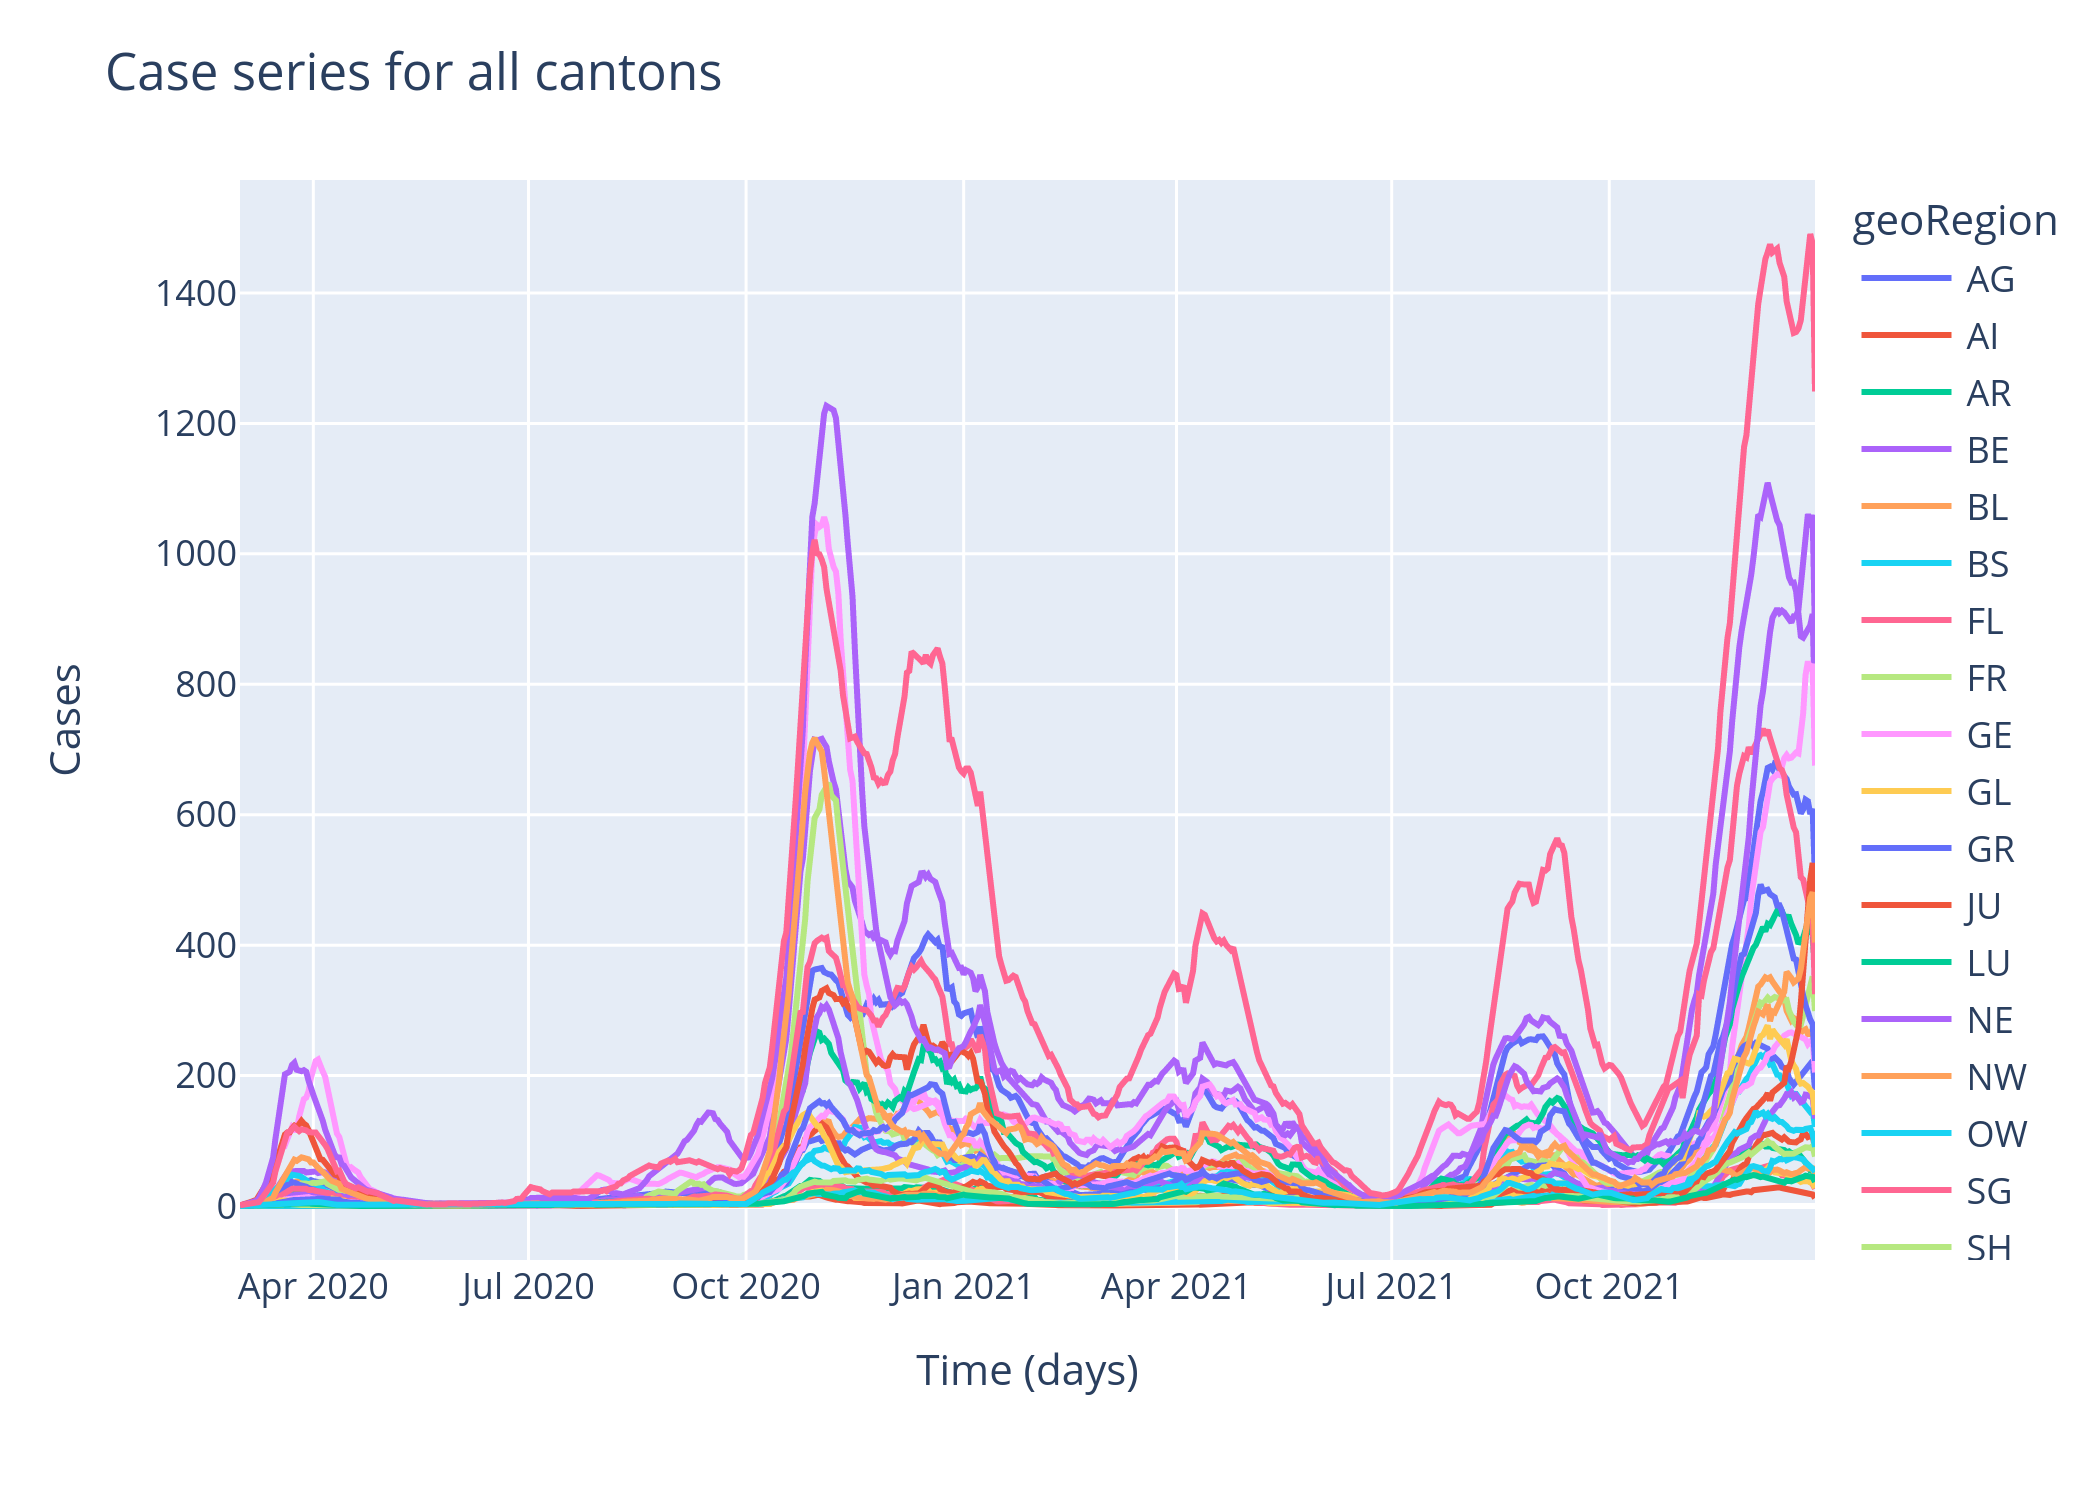
\includegraphics[width=\linewidth]{canton_series.png}
 % canton_series.png: 2100x1500 px, 72dpi, 74.08x52.92 cm, bb=0 0 2100 1500
 \caption{Timeseries of all cantons.}
 \label{fig:canton_series}
\end{figure}

    
    
    \hypertarget{calculating-the-cross-correlations}{%
\subsubsection{Calculating the
cross-correlations}\label{calculating-the-cross-correlations}}

If we take a closer look selected cantons we see that the most recent
wave started a little earlier on some cantons, relative to Geneva.
Notice that we also include the Vienna curve for reference.

From the curves in figure \ref{fig:lagged series}, we that there are substantial lags between some series especially between Vienna and Switzerland in the last wave. This feature gives us hope that we can use other series for predicting the evolution of incidence in some specific cantons.


\begin{figure}
 \centering
 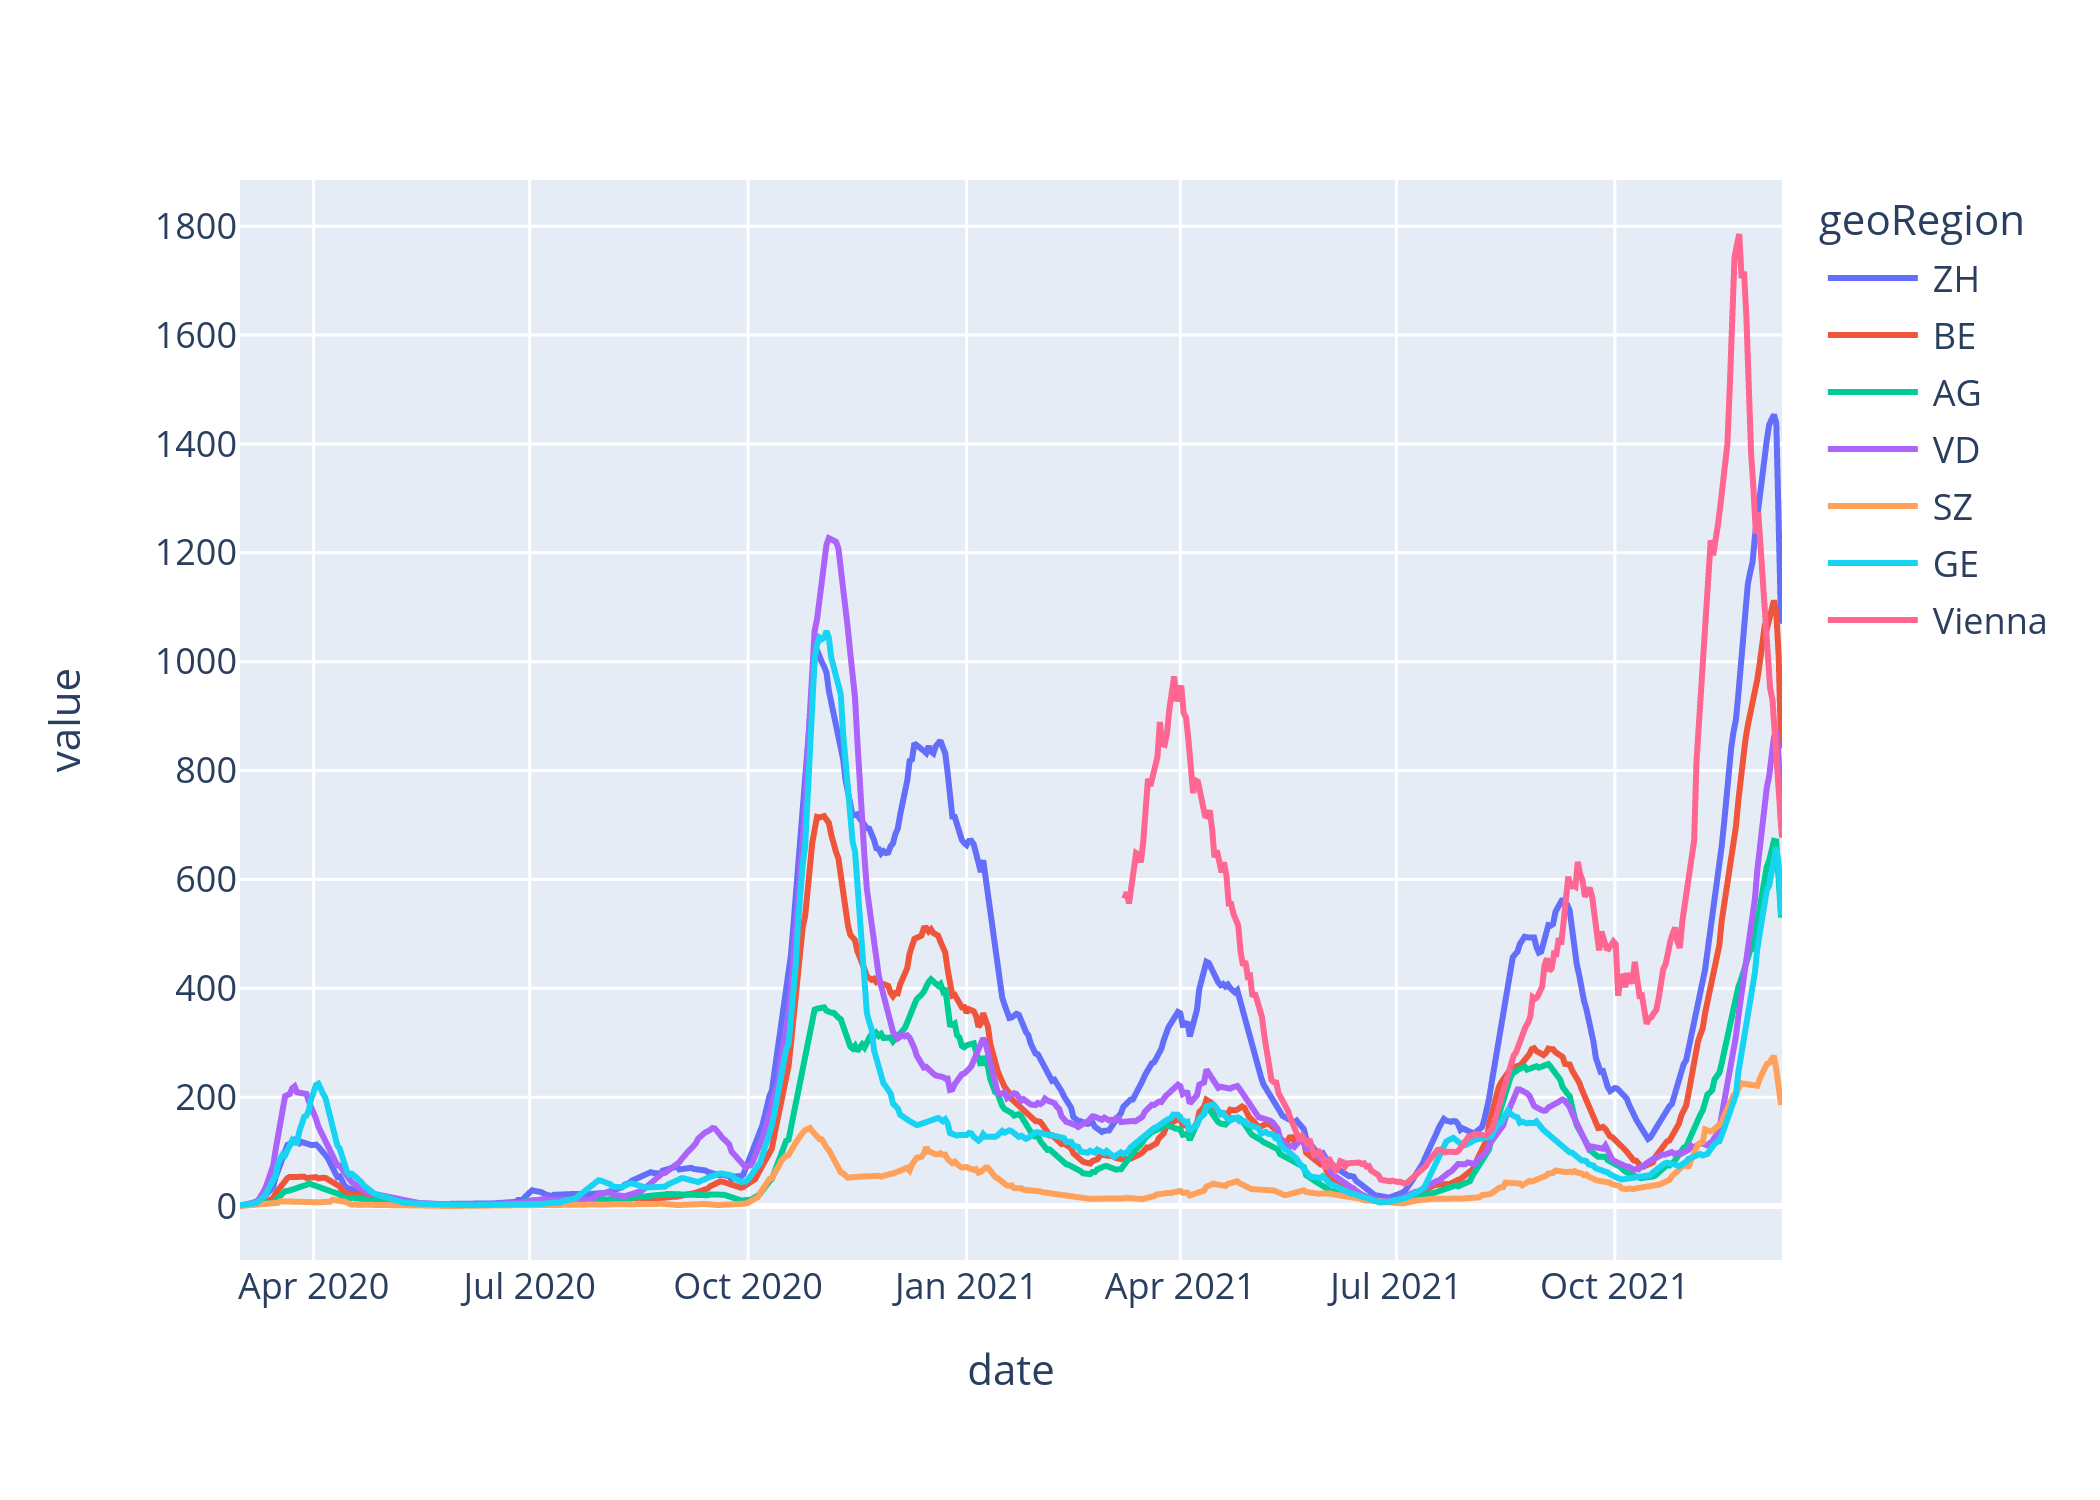
\includegraphics[width=\linewidth]{lagged_series.png}
 % lagged_series.png: 2100x1500 px, 72dpi, 74.08x52.92 cm, bb=0 0 2100 1500
 \caption{Selected Swiss cantons and Vienna.}
 \label{fig:lagged series}
\end{figure}


    
    
    
    
    It's even better to look at all pairwise cross-correlations (Figure \ref{fig:corr_matrix}).

\begin{figure}
 \centering
 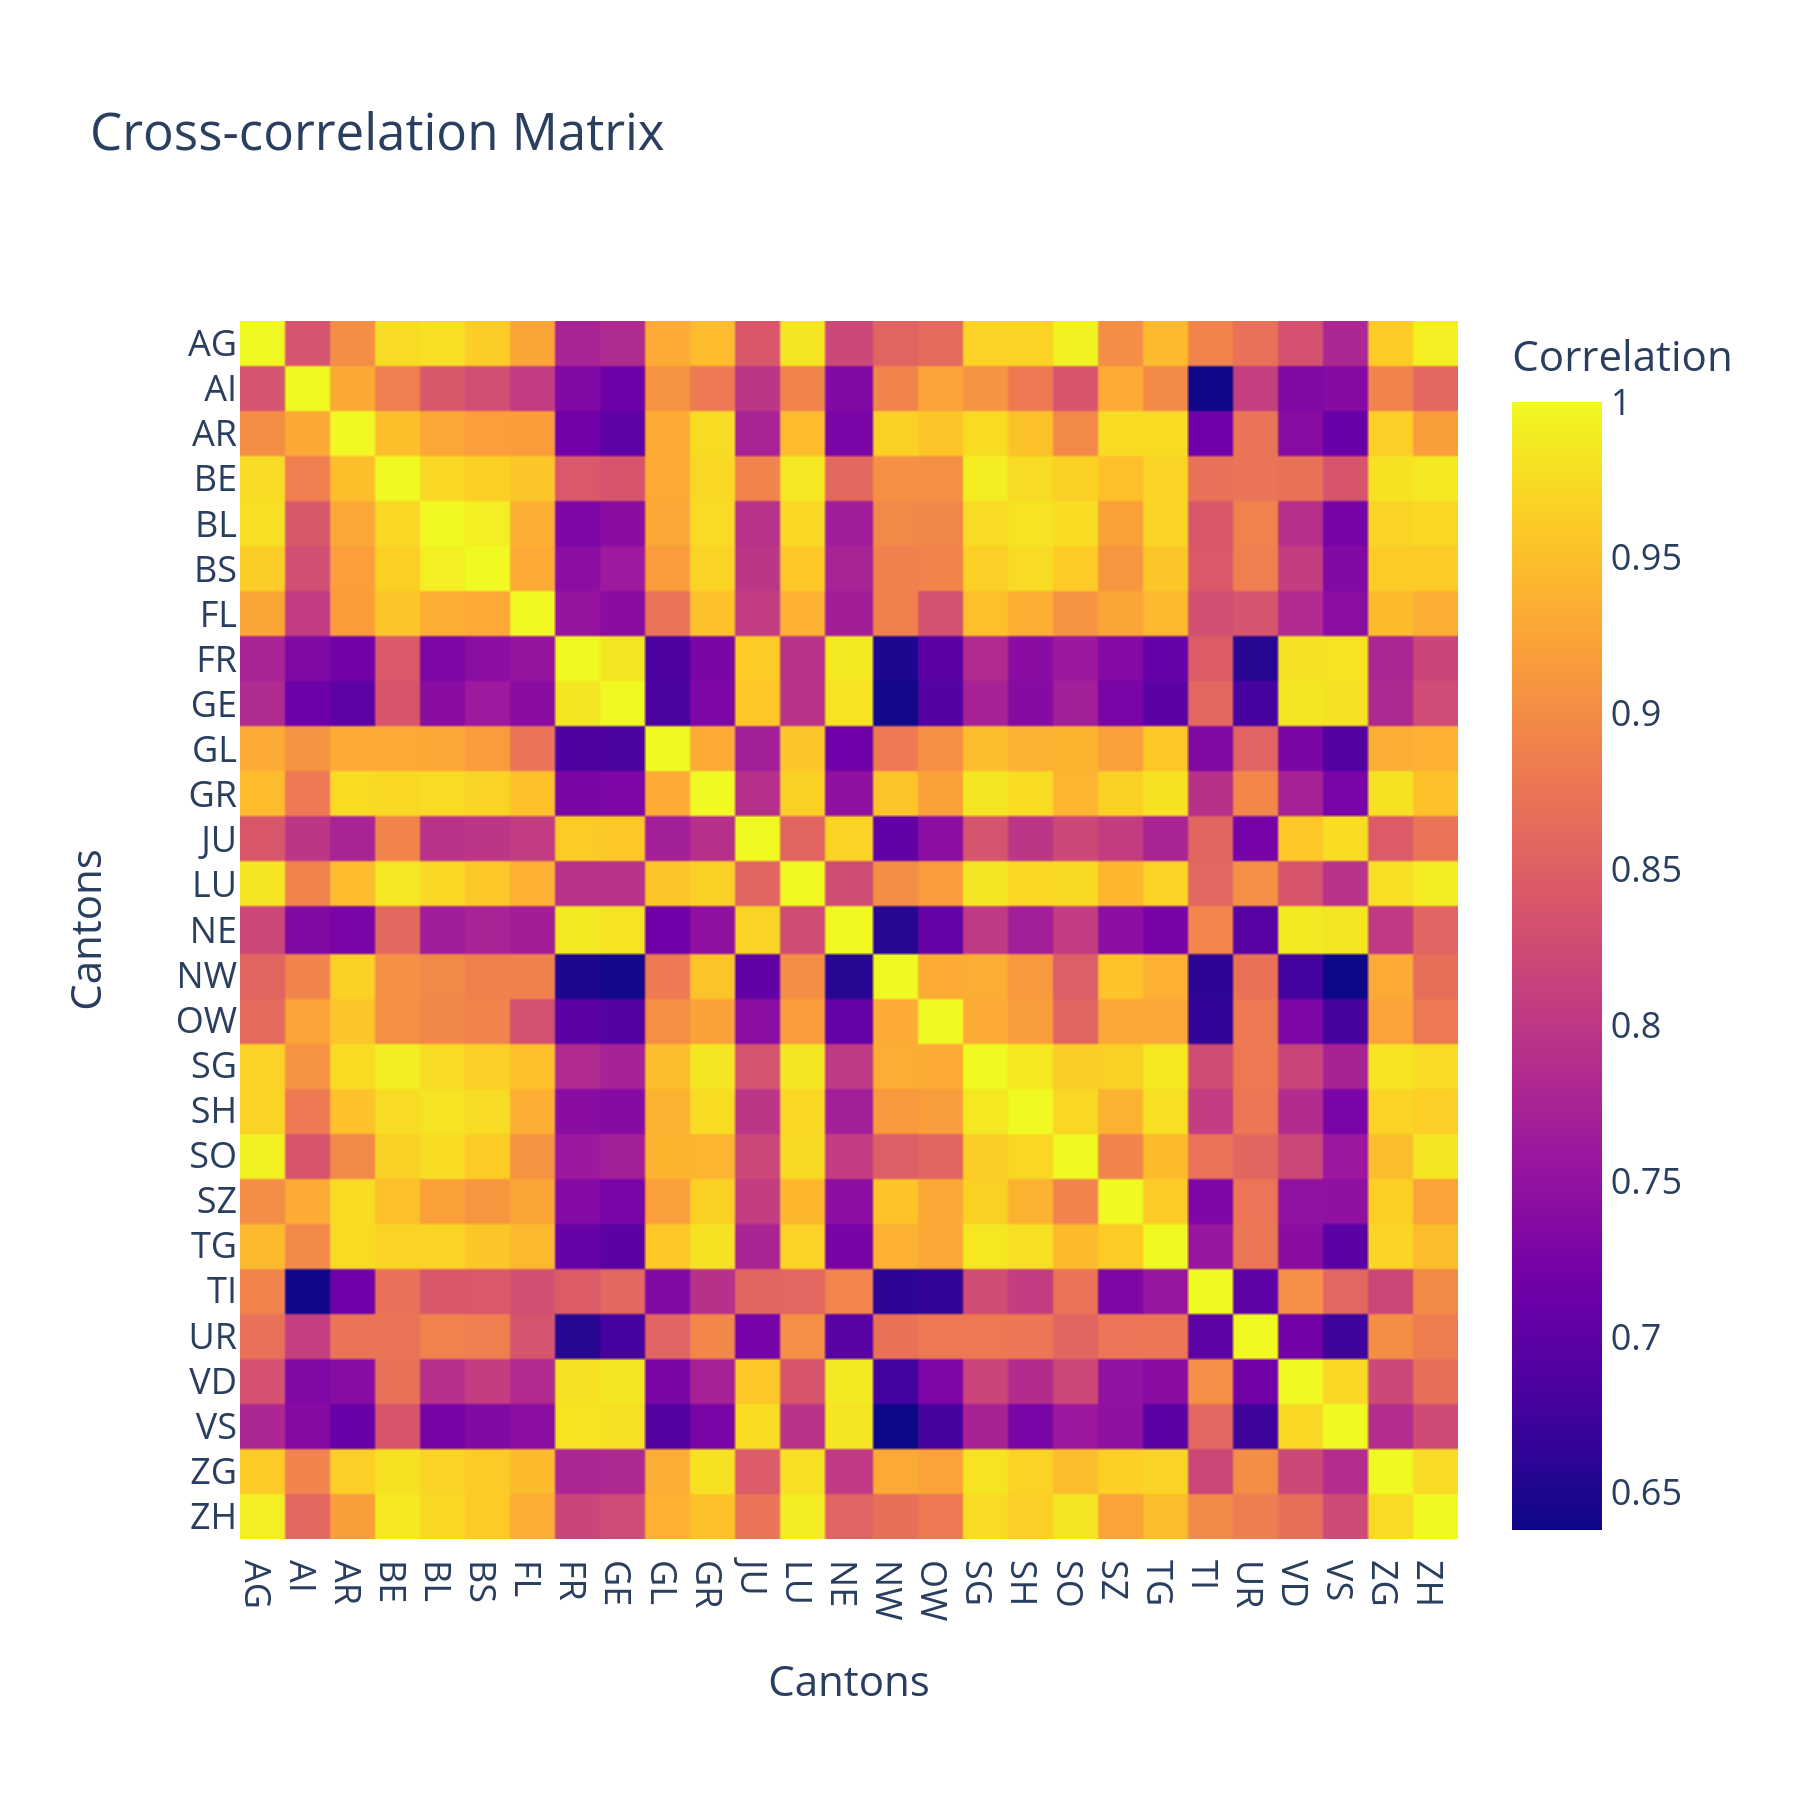
\includegraphics[width=\linewidth]{Cross-corr_matrix.png}
 % Cross-corr_matrix.png: 1800x1800 px, 72dpi, 63.50x63.50 cm, bb=0 0 1800 1800
 \caption{Correlation matrix between all cantons}
 \label{fig:corr_matrix}
\end{figure}
    
For each pair of Cantons there is also a lag which corresponds to their maximal correlation, which we can also represent in matrix form (Figure \ref{fig:lagmatrix}).

\begin{figure}
 \centering
 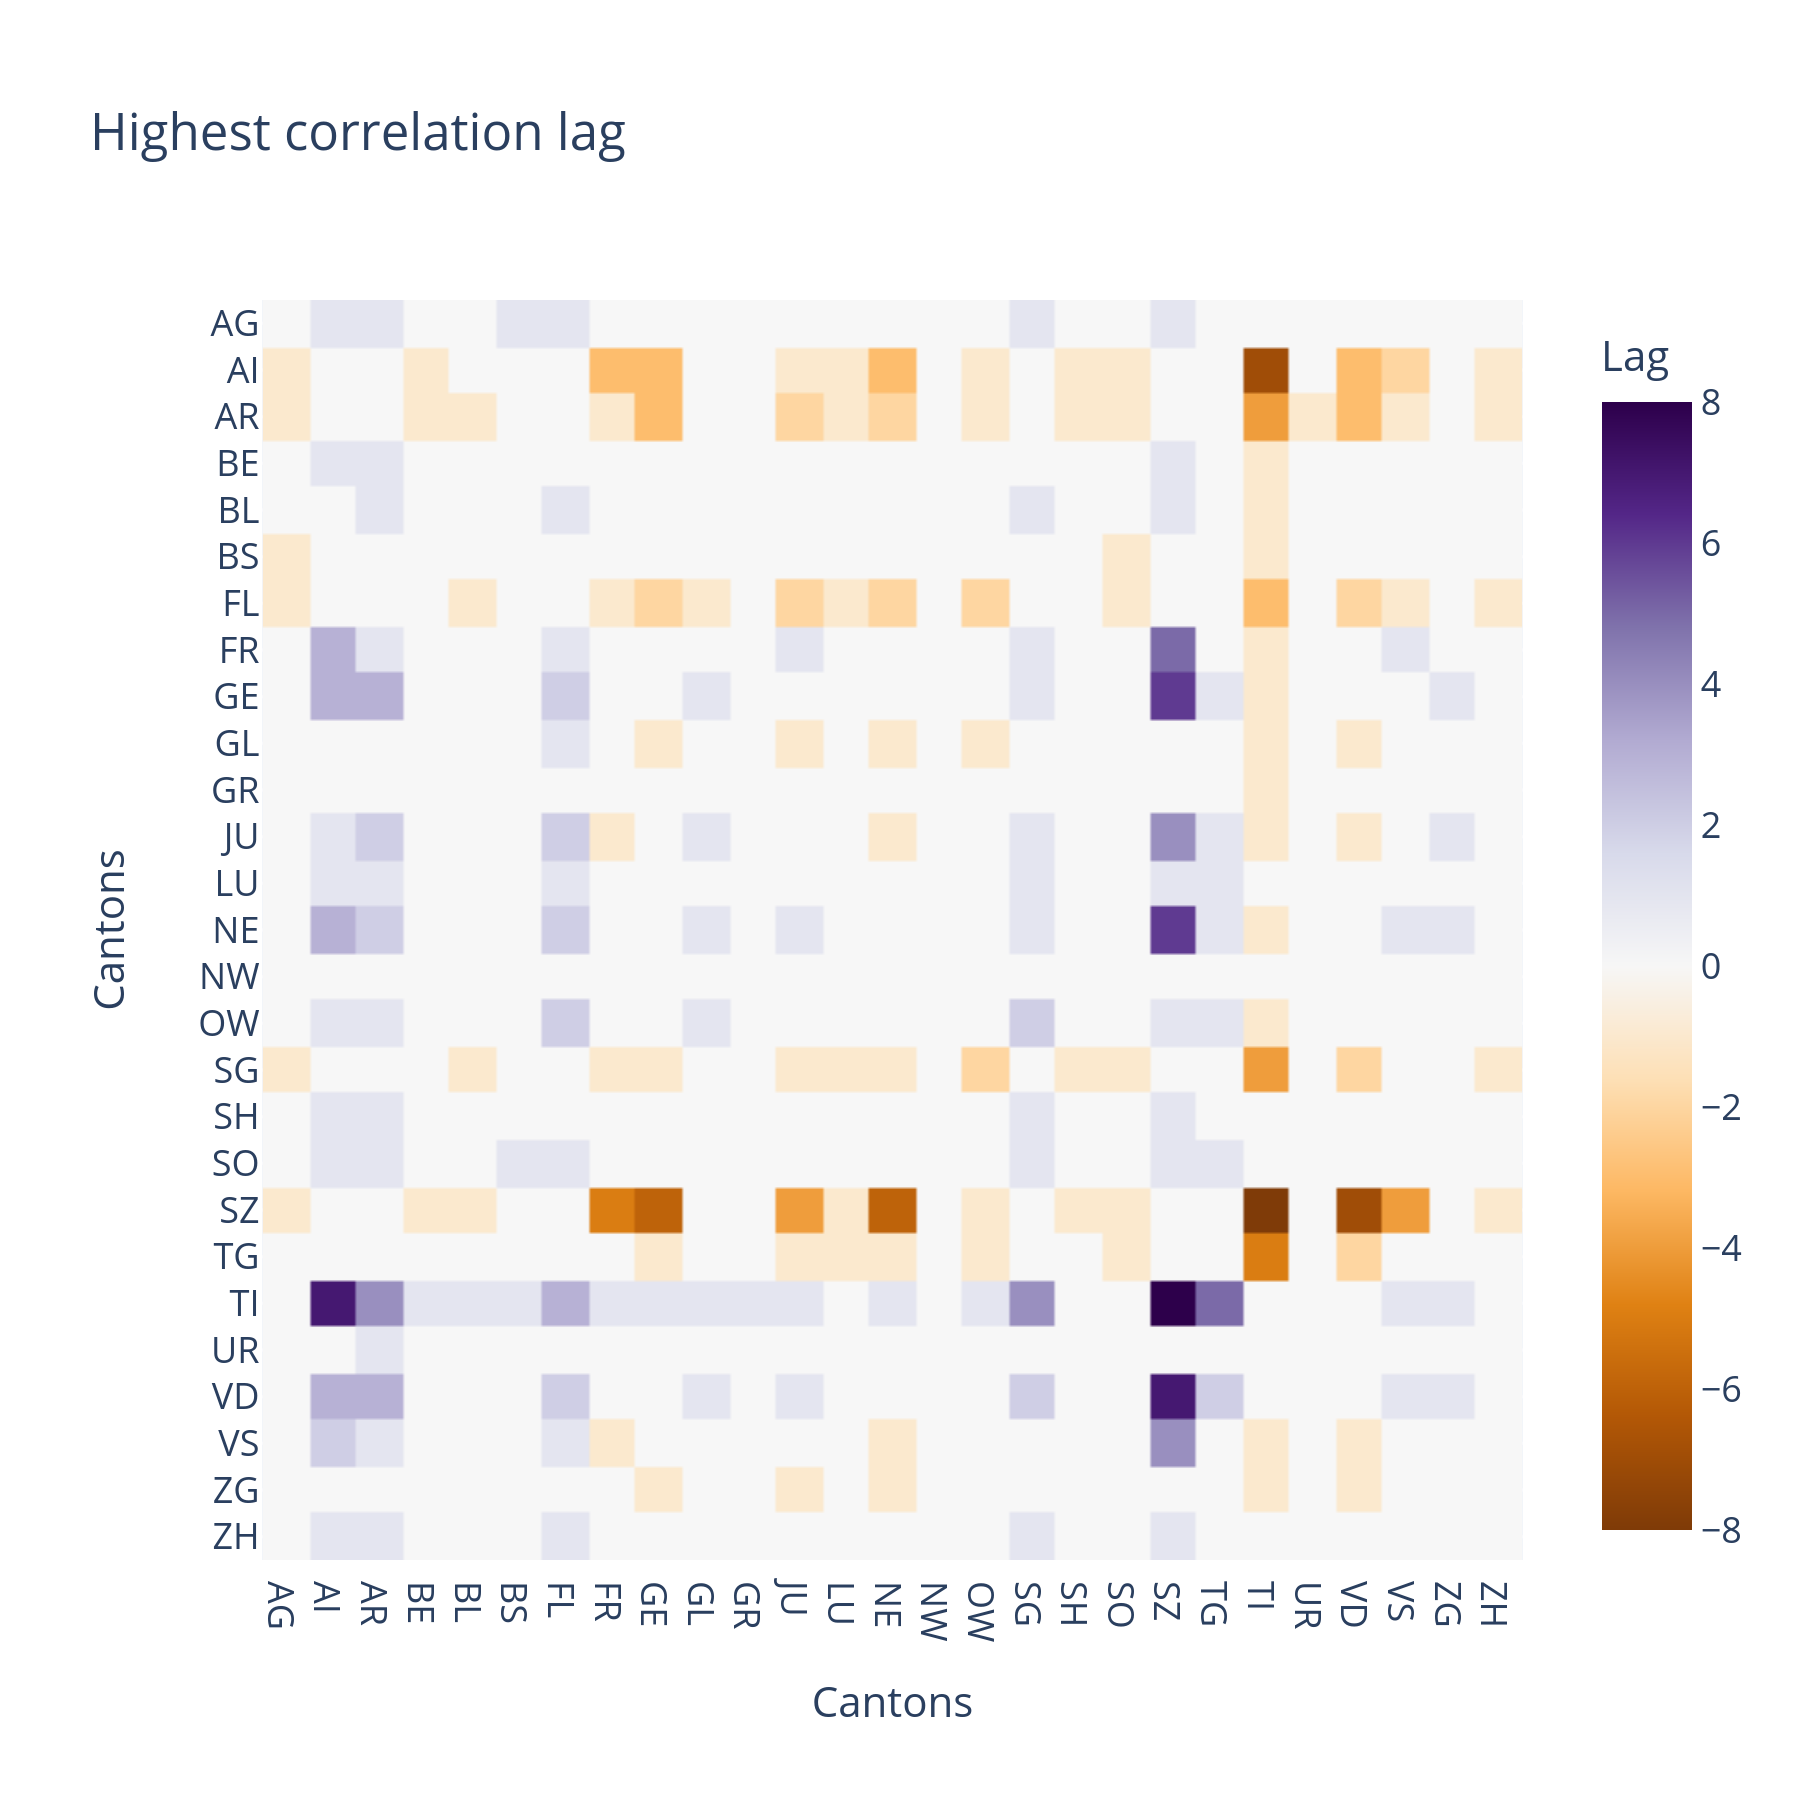
\includegraphics[width=\linewidth]{canton_lag_matrix.png}
 % canton_lag_matrix.png: 1800x1800 px, 72dpi, 63.50x63.50 cm, bb=0 0 1800 1800
 \caption{Pairwise lag matrix for all swiss cantons}
 \label{fig:lagmatrix}
\end{figure}

    
    
    \hypertarget{clustering-the-series-based-on-correlation}{%
\subsubsection{Clustering the Series based on correlation}\label{clustering-the-series-based-on-correlation}}

We can look at the cross-correlation as a measure of similarity between the time-series. Therefore we can use the correlation matrix, show in figure \ref{fig:corr_matrix}, as the basis of a hierarchical clustering algorithm.

\begin{figure}
 \centering
 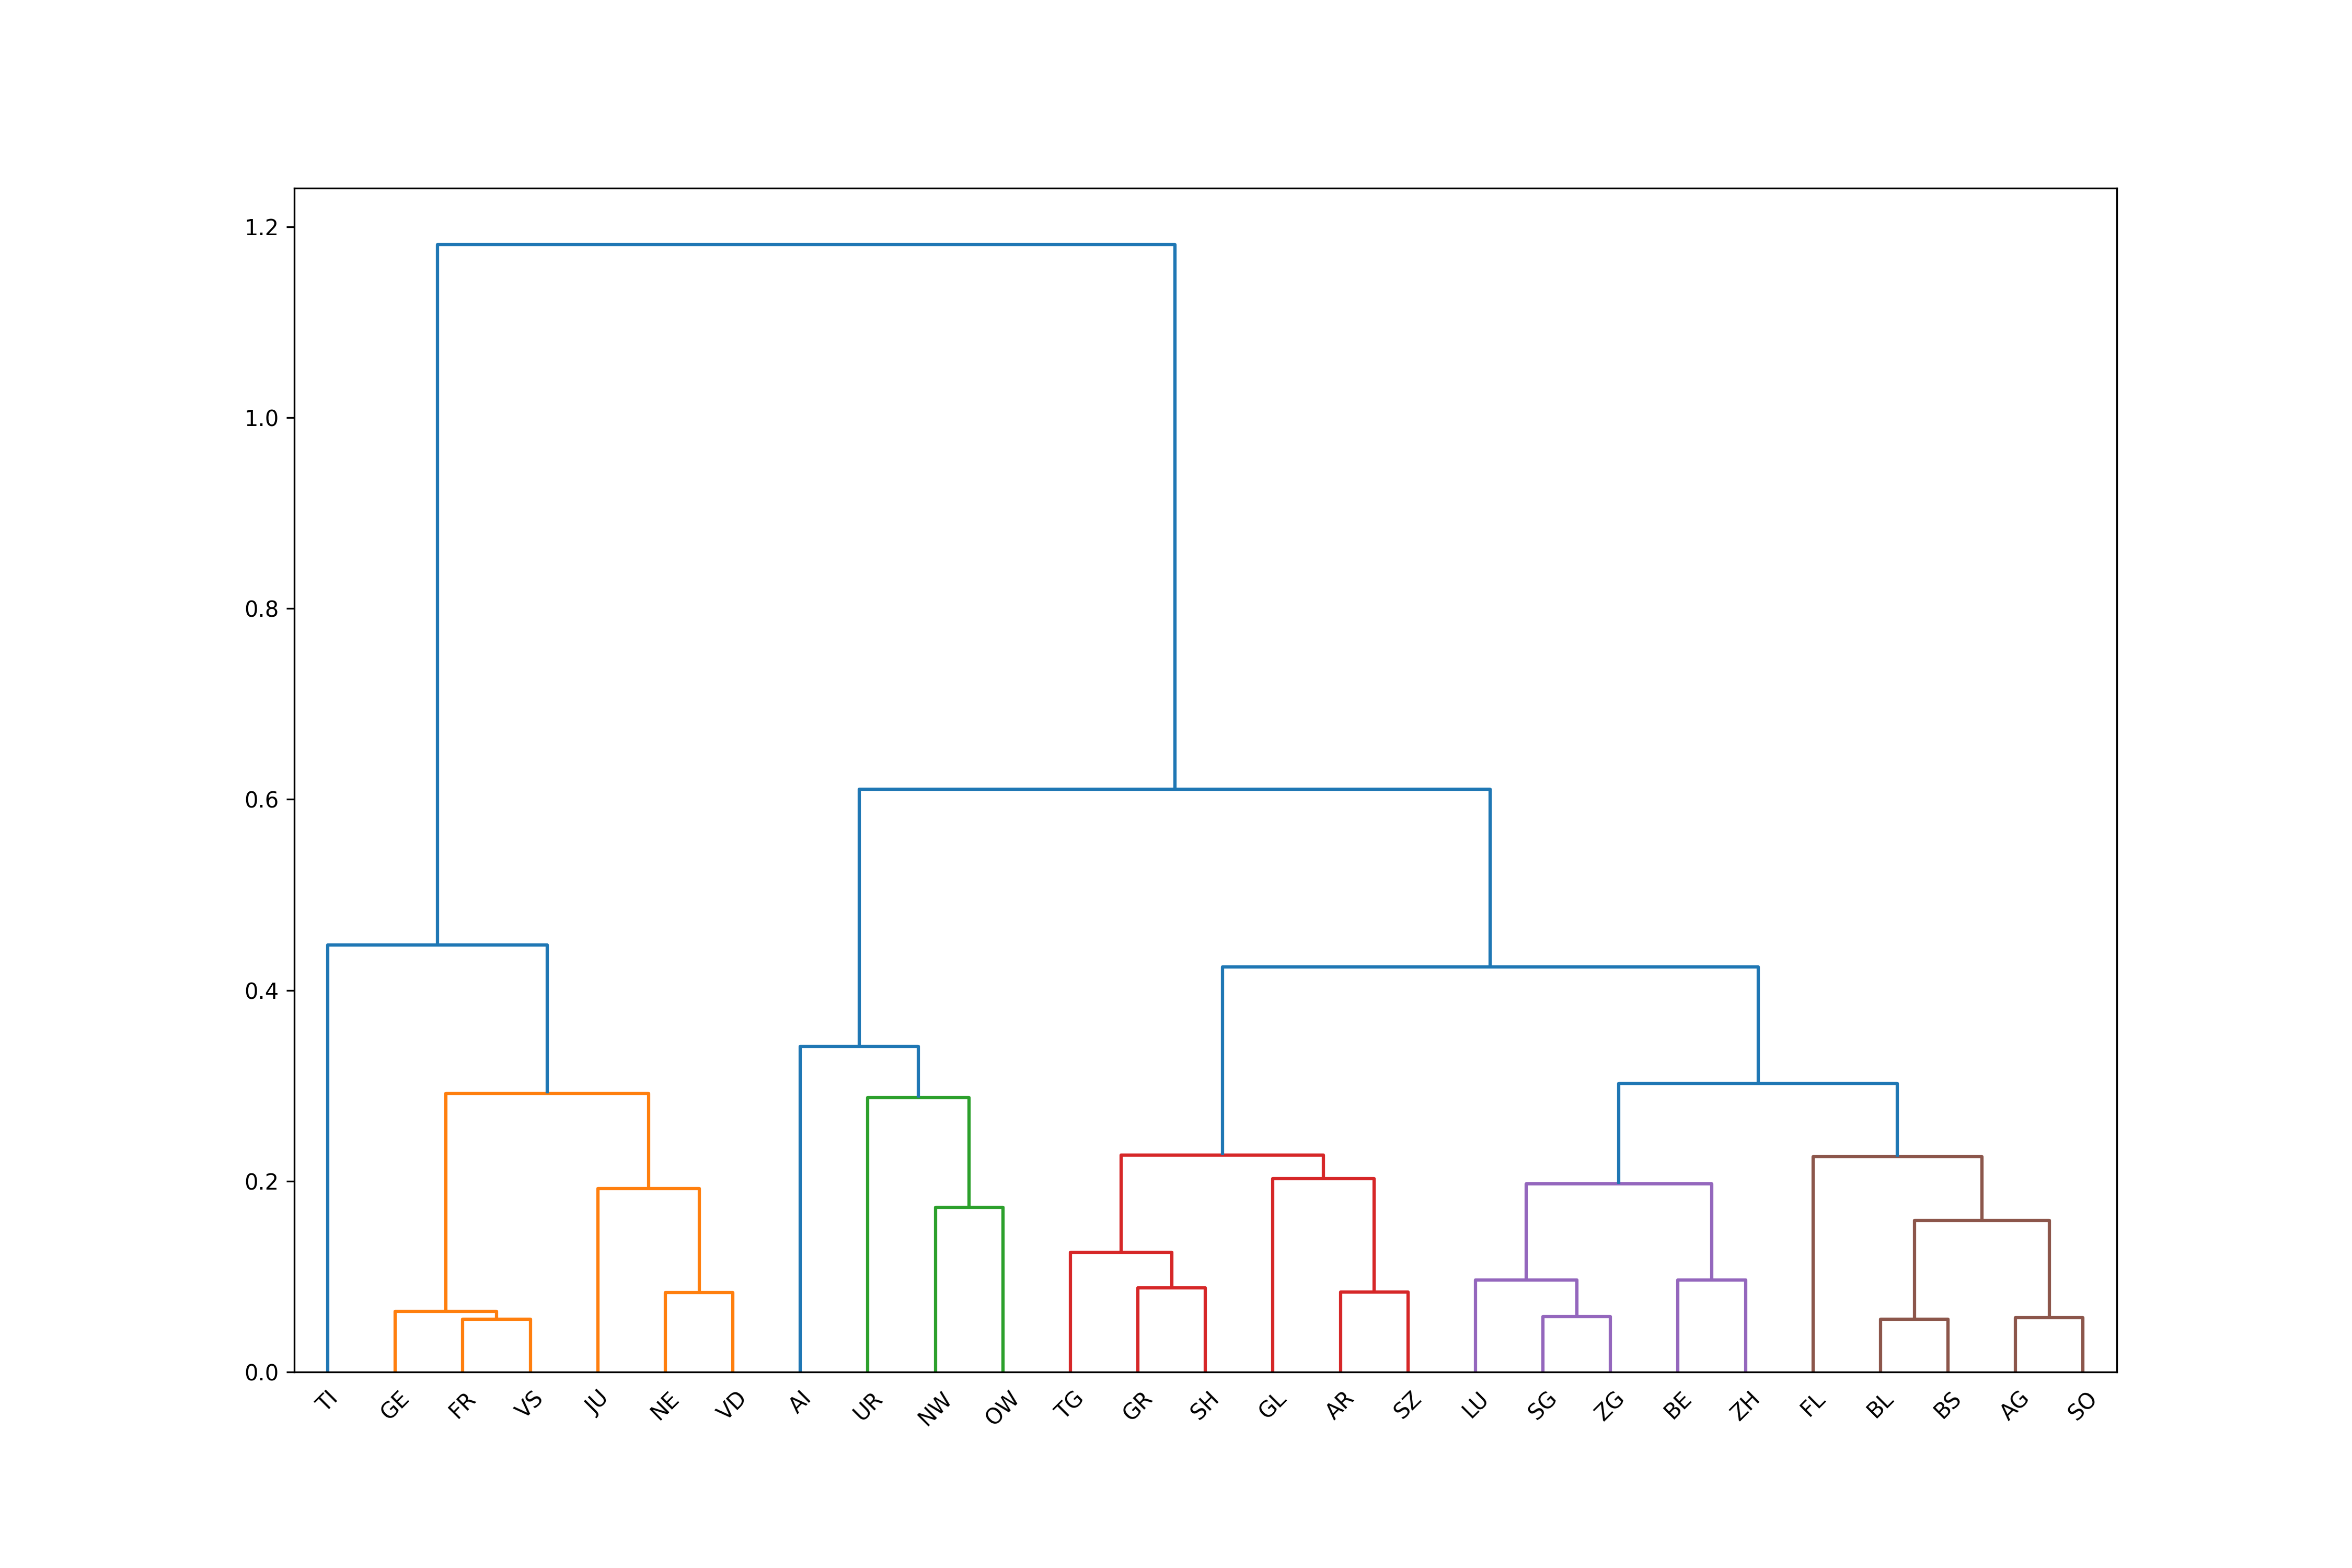
\includegraphics[width=\linewidth]{dendro.png}
 % dendro.png: 4500x3000 px, 300dpi, 38.10x25.40 cm, bb=0 0 1080 720
 \caption{Dendrogram with the results of the hierarchical clustering of the series.}
 \label{fig:dendro}
\end{figure}

\subsection{Geo visualization}\label{geo-visualization}

It might be informative to represent the lags  on a map of Switzerland.

\begin{figure}
 \centering
 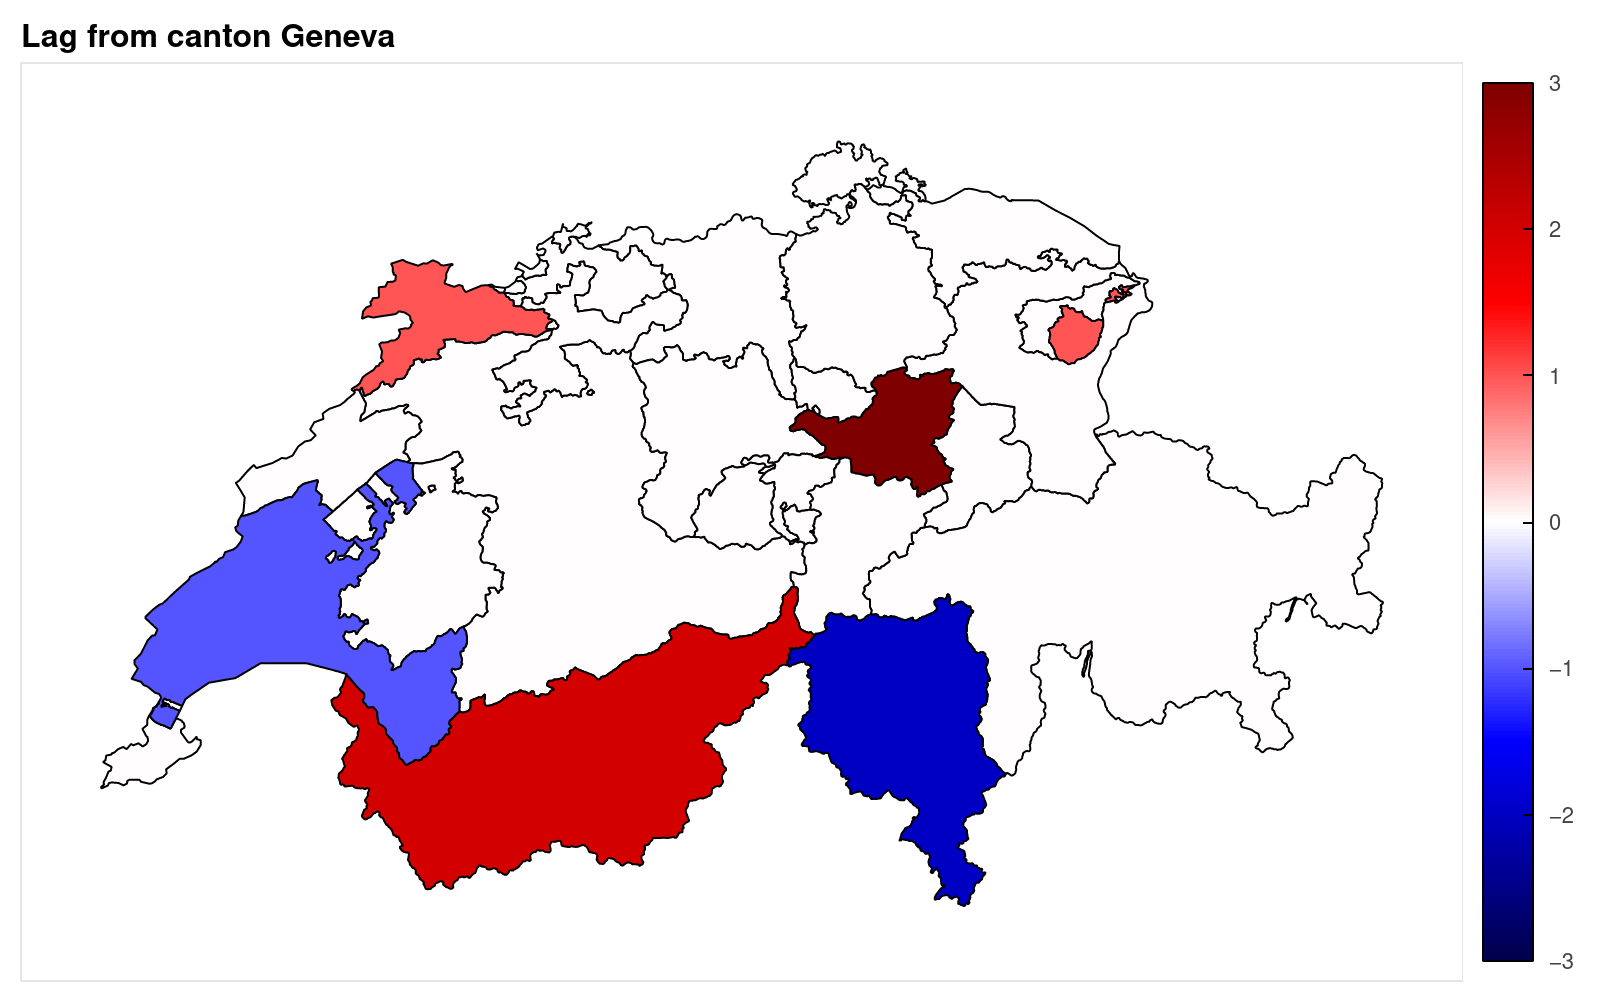
\includegraphics[width=\linewidth]{map_lags.png}
 % map_lags.png: 1600x1000 px, 72dpi, 56.44x35.28 cm, bb=0 0 1600 1000
 \caption{Map of Switzerland colored by the magnitude of the lags relative to canton Geneva. Lag scale is in days.}
 \label{fig:maplags}
\end{figure}

    

        
    \hypertarget{network-analysis}{%
\subsubsection{Network analysis}\label{network-analysis}}

We can take the correlation matrix and build a network to represent the
association between the cantons. for this network we will filter only
correlations greater than \(0.7\). We will use the correlation as the
weight of each edge in the network. These weights can be used 

    
    
\begin{figure}
 \centering
 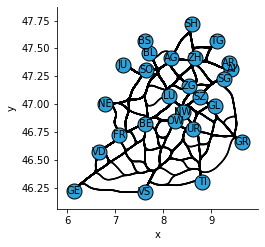
\includegraphics[width=\linewidth]{net_communities.png}
 % net_communities.png: 1600x1000 px, 72dpi, 56.44x35.28 cm, bb=0 0 1600 1000
 \caption{Communities detected on the network of cantons.}
 \label{fig:network}
\end{figure}
    
 
        
    \hypertarget{bayesian-inference}{%
\subsection{Bayesian Inference}\label{bayesian-inference}}

If we think about Epidemic as stochastic processes, it may be worth to try to infer some basic rates of this process from the data.

We start by restricting our observations to 2021, to avoid a potentially different dynamics in the beginning of the pandemic.  

    \hypertarget{cases-and-hospitalizations-as-binomial-processes-with-variable-rates}{%
\subsubsection{Cases and Hospitalizations as Binomial processes with
variable
rates}\label{cases-and-hospitalizations-as-binomial-processes-with-variable-rates}}

If we treat cases and hospitalizations as bionomial processes, we can
estimate their variable rates. From the Test series, \(T_t\) we can
model the prevalence series in the population,
\(Pv_t \sim Beta (\alpha, \beta)\) as

\[Cases_t \sim Bin(n=T_t, p=Pv_t).\]

In a similar fashion, we can model the probability of Hospitalization,
\(Ph_t \sim Beta (\alpha, \beta)\) as

\[Hospitalizations_t \sim Bin(n=Cases_t, p=Ph_t).\]



The diagram of our inference looks like the figure below:
 
            
    
    \begin{center}
    \adjustimage{max size={0.9\linewidth}{0.9\paperheight}}{Bayesian Hosp. rate_files/Bayesian Hosp. rate_95_0.pdf}
    \end{center}
    { \hspace*{\fill} \\}
    

    Which after our estimation yields the following posterior probability distribution
 for the prevalence over time (Figure \ref{fig:prev}). Notice that it matches quite well the test
positivity data (purple dots).

The posterior distribution of the probability of Hospitalization for positive cases is shown in figure \ref{fig:phosp}

    
\begin{figure}
 \centering
 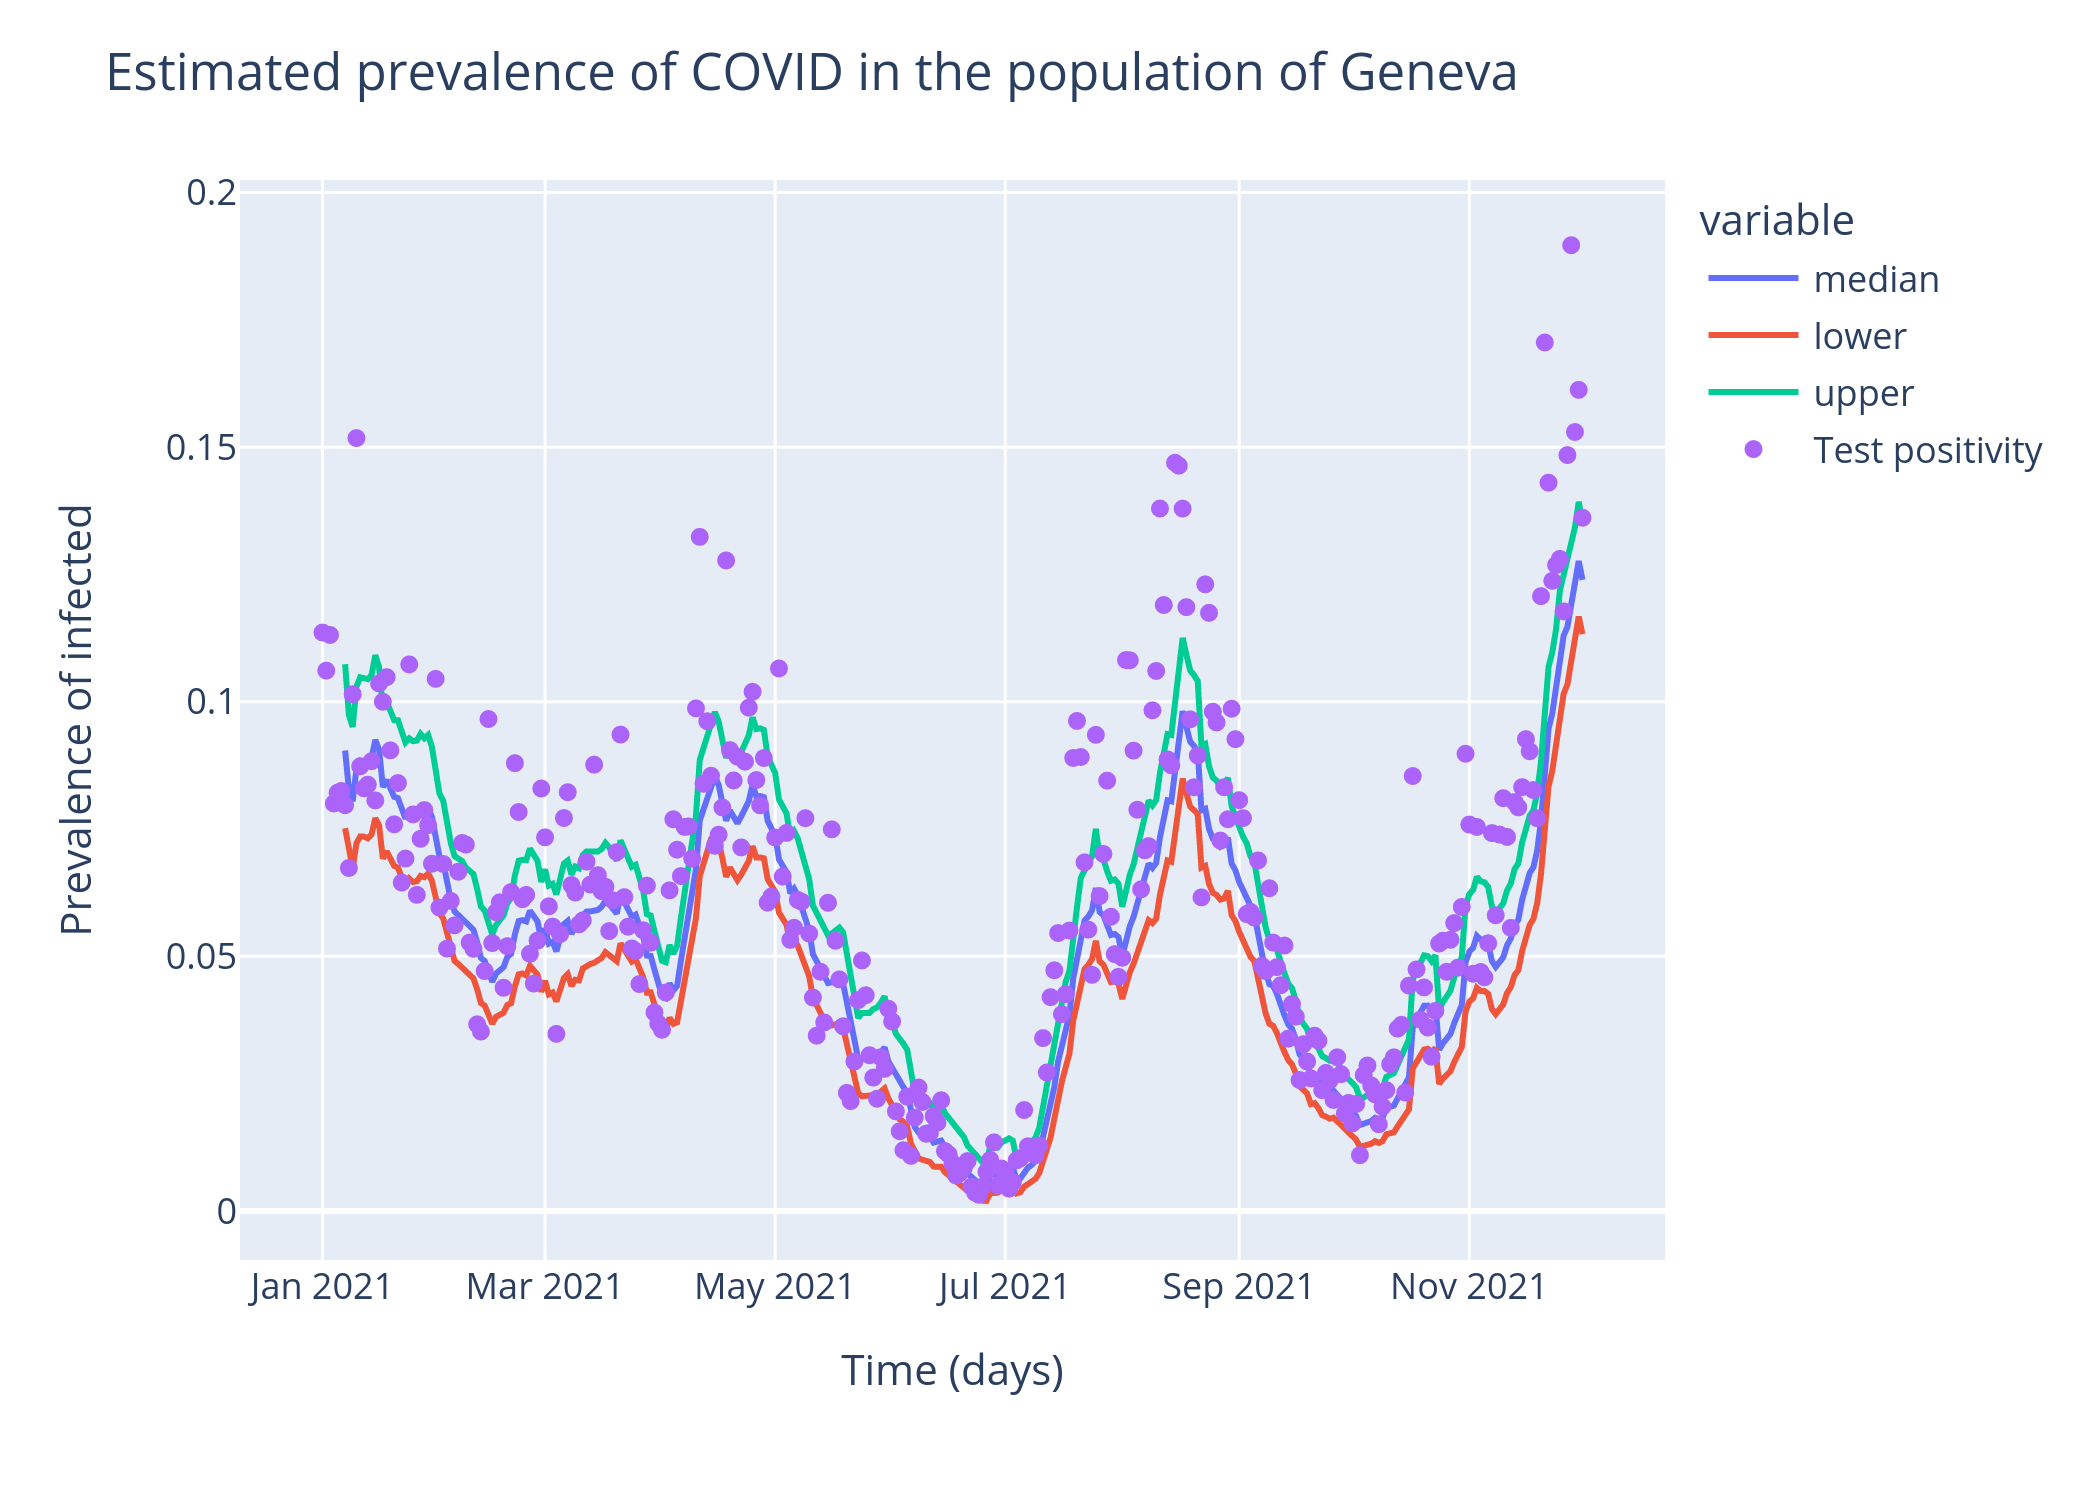
\includegraphics[width=\linewidth]{prevalence_est.png}
 % prevalence_est.png: 2100x1500 px, 72dpi, 74.08x52.92 cm, bb=0 0 2100 1500
 \caption{Estimated prevalence of covid cases as a fraction of the exposed population. Estimated median and 95\% credible bounds are shown as a 7-day moving average.}
 \label{fig:prev}
\end{figure}

\begin{figure}
 \centering
 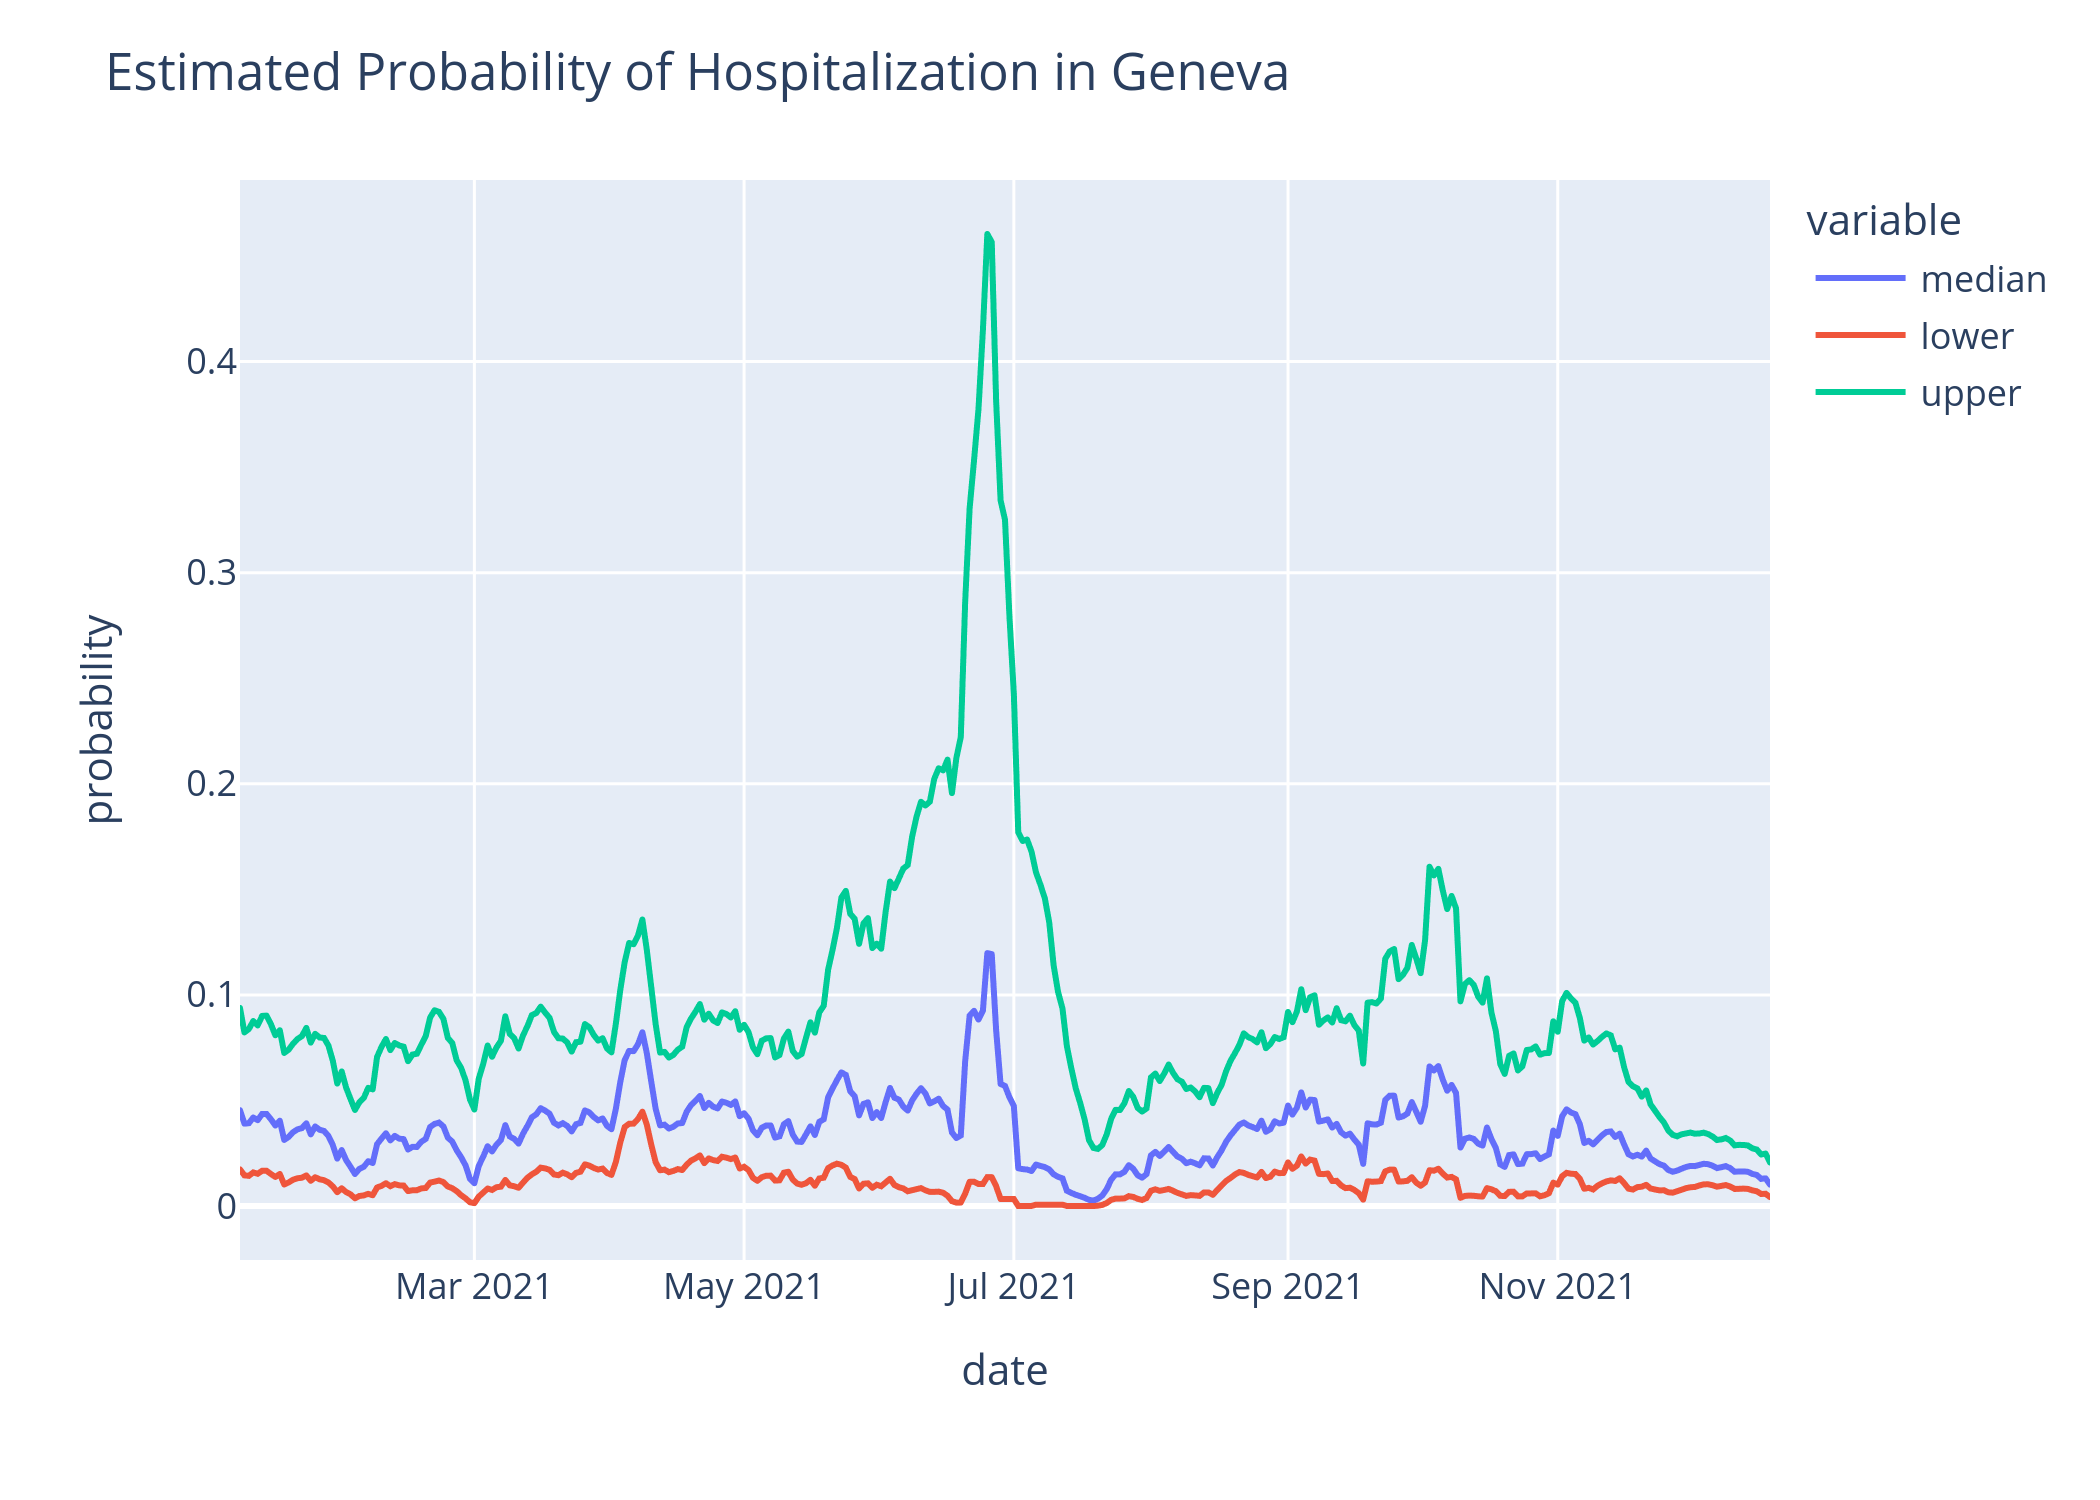
\includegraphics[width=\linewidth]{phosp.png}
 % phosp.png: 2100x1500 px, 72dpi, 74.08x52.92 cm, bb=0 0 2100 1500
 \caption{Posterior probability distribution for the probability of Hospitalization.}
 \label{fig:phosp}
\end{figure}

    
    \hypertarget{sir-based-forecasting}{%
\subsubsection{SIR-based Forecasting}\label{sir-based-forecasting}}

The FOPH makes available the daily estimates of the effective
reproductive number, $R_t$. With a good estimate of $R_t$ it is possible
to simulate growth based on transmission models. Since for the SIR
model, \[R_t = R_0 S(t)= \frac{\beta}{\gamma}S(t),\] we can use it to
parameterize a simple transmission model with which to forecast cases and
thus hospitalizations. We would normally write the SIR model as:

\begin{align}
\frac{dS}{dt} &= -\beta S(t)I(t)\\
\frac{dI}{dt} &= \beta S(t)I(t) -\gamma I(t)
\end{align}

From the $R_t$ time series, we can derive a time-dependent
transmission parameter, \[\beta(t)=\frac{R_t \gamma}{S(t)}.\]

Then we can re-write the SIR model as

\begin{align}
\frac{dS}{dt} &= -R_t\gamma I(t)\\
\frac{dI}{dt} &= R_t\gamma I(t) -\gamma I(t) \label{eq:I}
\end{align}

We can reduce the system above to just equation \ref{eq:I}, which has
the following solution:

\[I(t) = I(0) e^{(R_t-1)\gamma t}\]

The \emph{prevalence} in the population that we estimated before, in the
SIR model is given by \(I(t)\). We can see that its evolution is
dependent of the effective reproductive number, and our ability to
forecast it. We can also easily propagate the uncertainty of the \(R_t\)
estimate to obtain uncertainty bands for I(t) as well.

    Let's apply this inference just to the last wave starting on october,
15th. To facilitate the fit to the model let's also use the 7-day moving
average of it.

    
    

    The structure of the probabilistic model is depicted below.
 
            
    
    \begin{center}
    \adjustimage{max size={0.9\linewidth}{0.9\paperheight}}{Bayesian Hosp. rate_files/Bayesian Hosp. rate_106_0.pdf}
    \end{center}
    { \hspace*{\fill} \\}
    

After we run the inference, we obtain posterior distributions for all parameter in the diagram above which are shown below.
        
    \begin{center}
    \adjustimage{max size={0.9\linewidth}{0.9\paperheight}}{Bayesian Hosp. rate_files/Bayesian Hosp. rate_109_0.png}
    \end{center}
    { \hspace*{\fill} \\}
    
I call attention to the the \textit{gamma} parameter, which is the recovery rate of infected individuals, corresponding to a recovery period of approximately 5 days ($1/\gamma)$.

We also get a posterior distribution for the prevalence curve ($I(t)$)

\begin{figure}
 \centering
 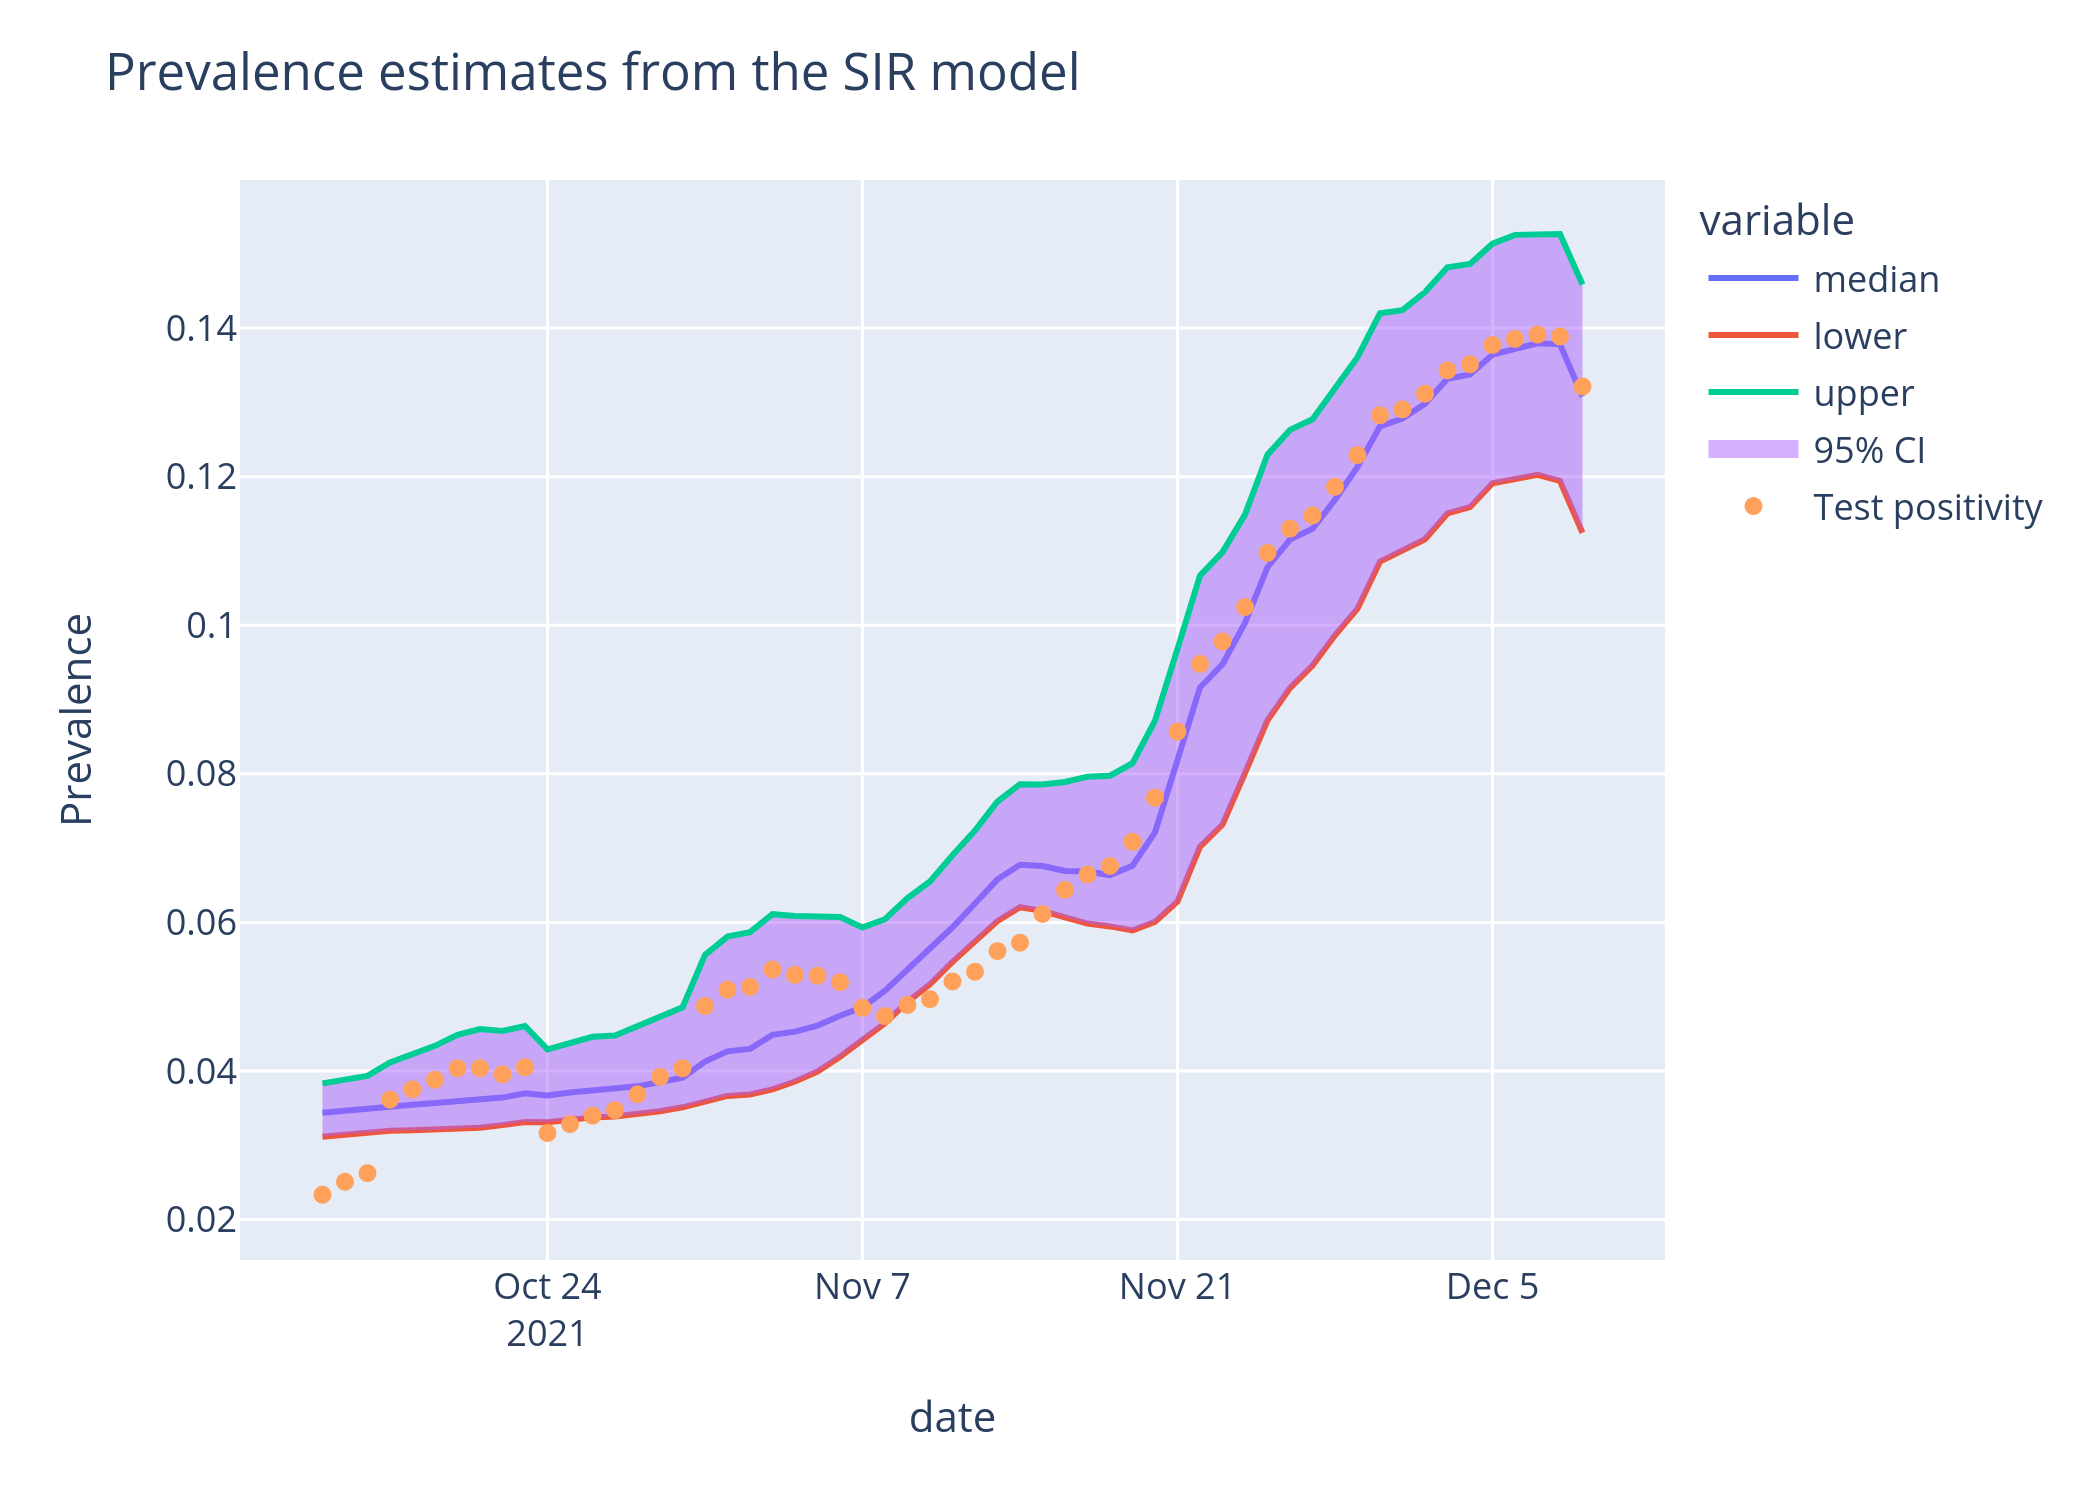
\includegraphics[width=\linewidth]{SIR_bayes.png}
 % SIR_bayes.png: 2100x1500 px, 72dpi, 74.08x52.92 cm, bb=0 0 2100 1500
 \caption{Posterior distribution for the model-based prevalence curve. Observed prevalence is represented as orange dots.}
 \label{fig:sir}
\end{figure}

    
    \hypertarget{forecasting}{%
\subsection{Forecasting}\label{forecasting}}

Statistical forecasting models can also be quite useful to forecast trend in time-series. In the particular case of our dataset, since we want to make full use of all available data, including the series of cases and hospitalizations from other cantons beloging to the same canton we are interested in forecasting, we end up with a pretty large matrix of predictor that need to be properly weighted to achieve optimal results.

For this purpose evaluated two Machine-learning models to Forecasting, namely K-nearest-neighbor regression (KNN) and Gradient Boosting Machine (LightGBM). The latter is in itself an ensemble of piecewise regressions which are fitted to the subsets of the data, minimizing a Mean-squared loss function. Both models are non-parametric and quite robust with respect to non-gaussian data. The LightGBM, model also includes automatically variable selection.

For both models the regression is defined as 

    $$H_{k,t} \sim C_{k,t-\tau_i} + H_{k,t-\tau_i} +V_{k,t-\tau_i},$$
    
Where $\tau$ takes values from the sequence $[1,2,\ldots 14]$, and k takes values from the set of cantons from the same cluster of the Canton we are forecasting for.

\begin{figure}
\centering
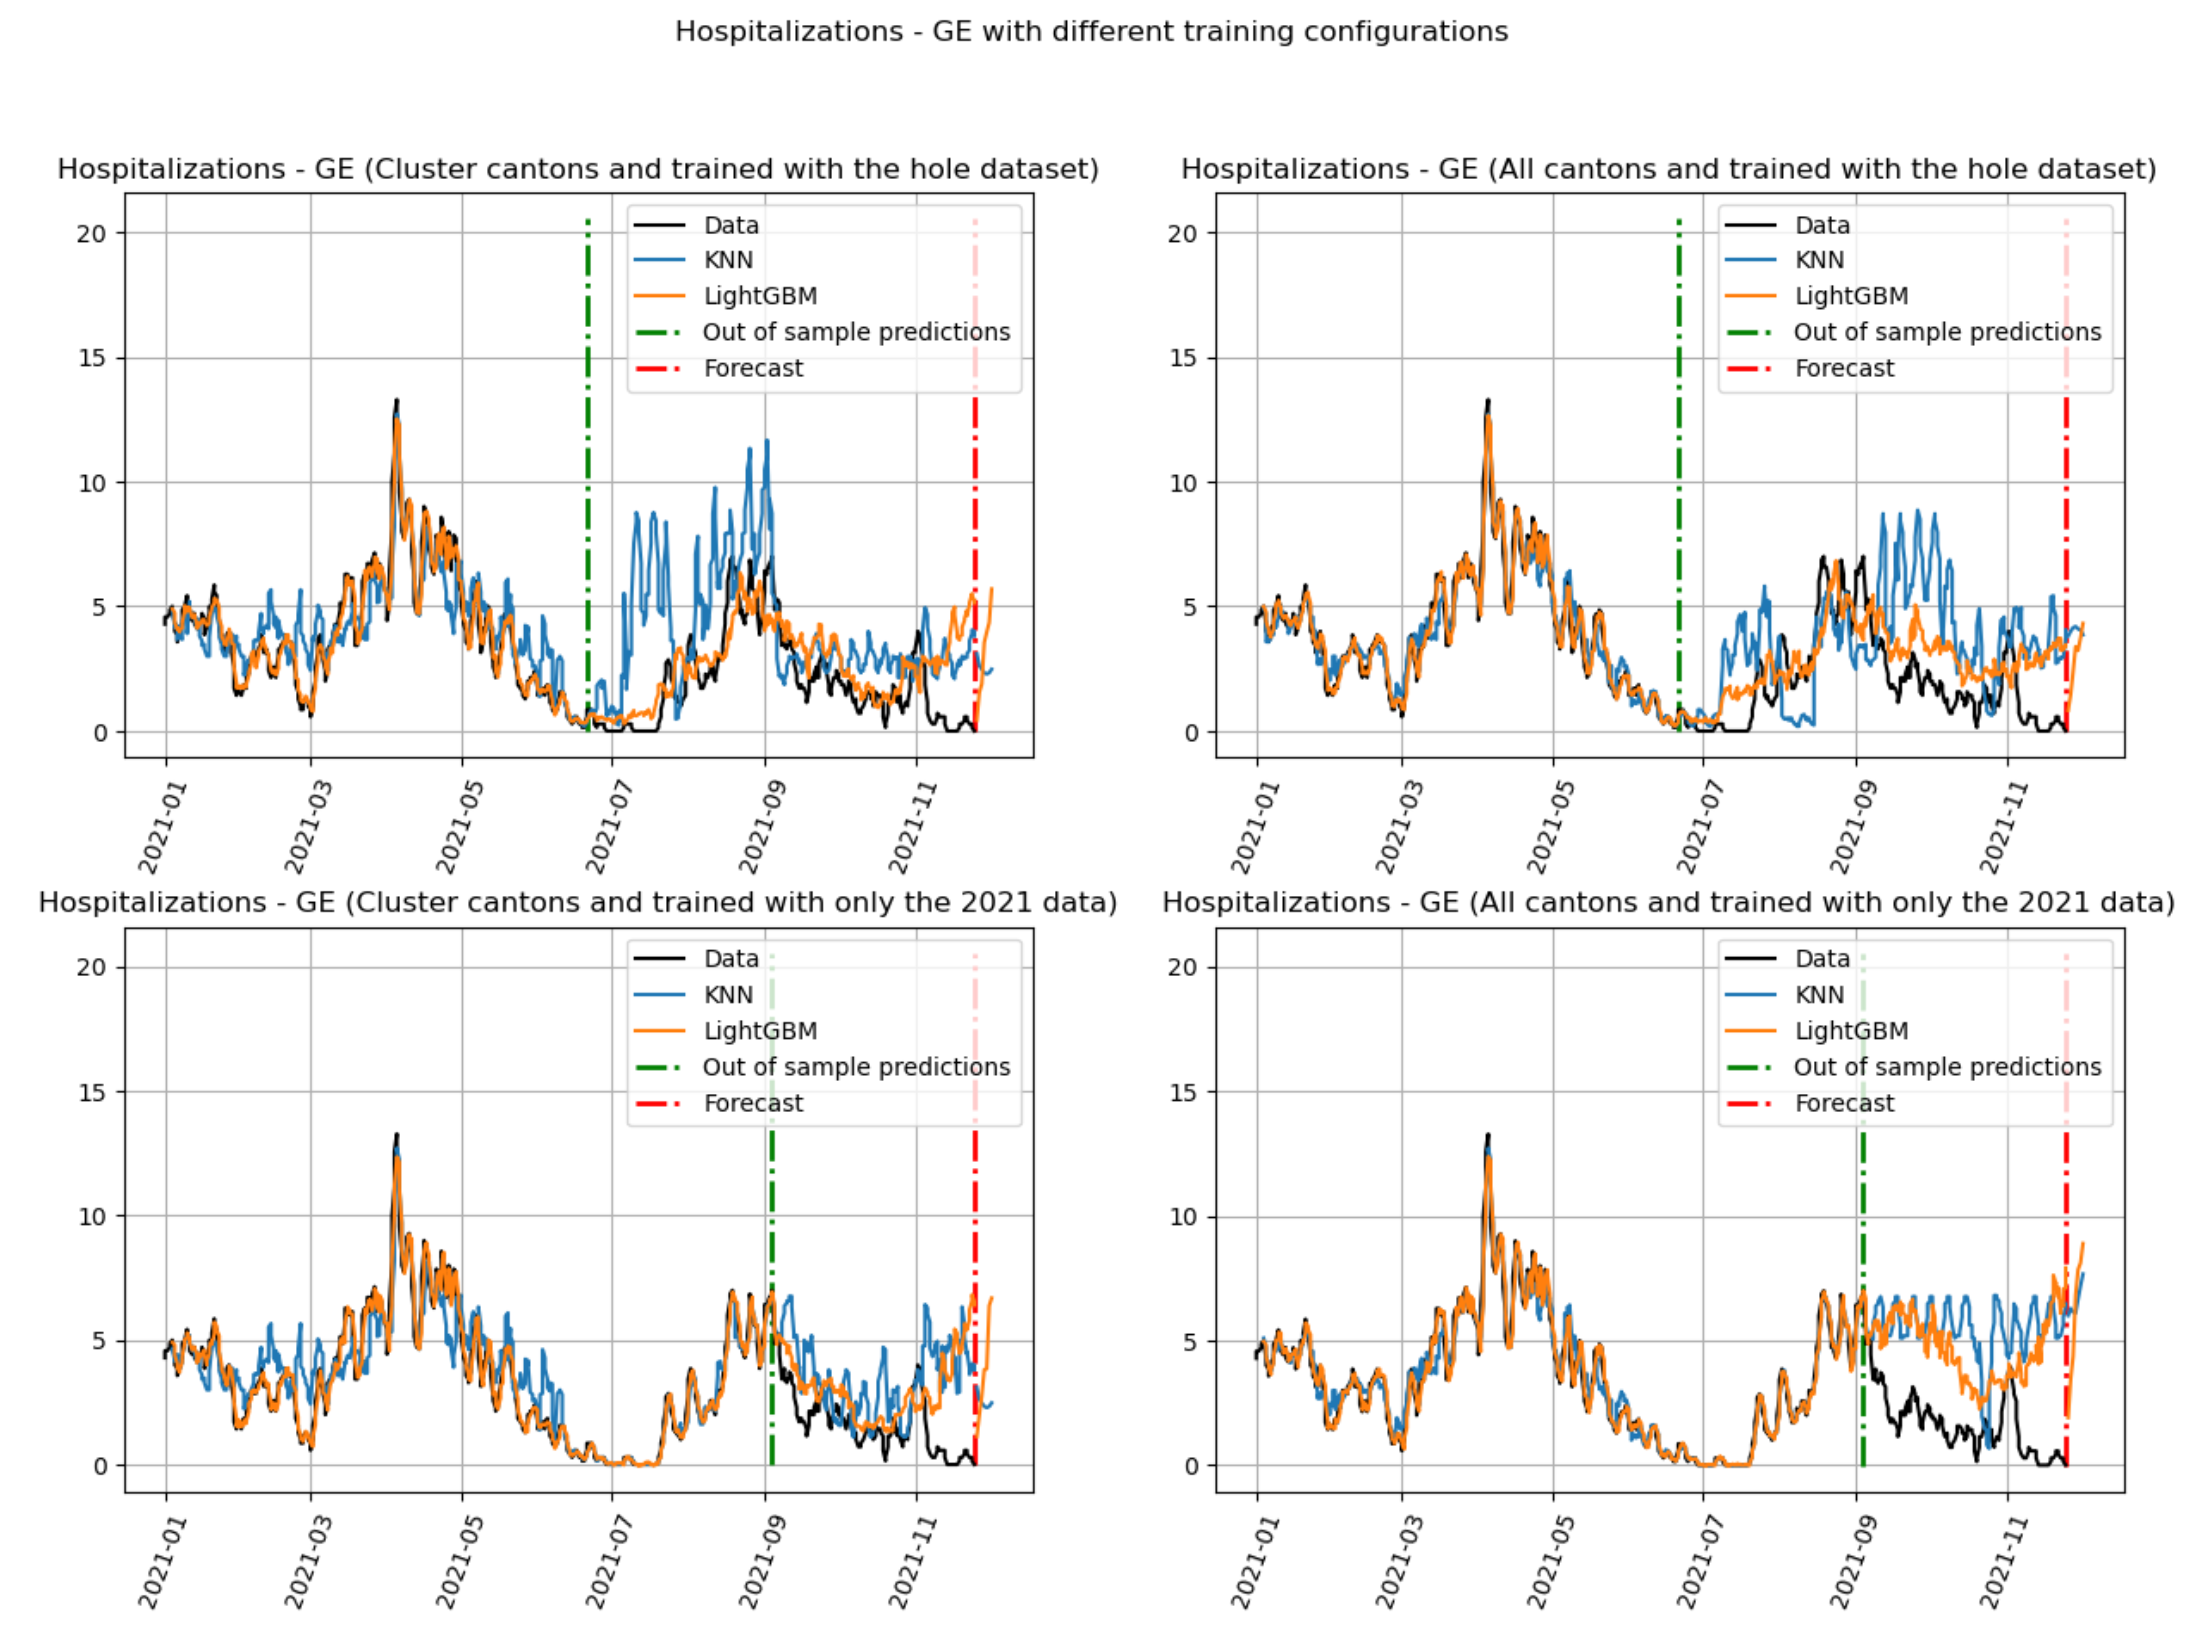
\includegraphics{forecasts.png}
\caption{forecasts}
\end{figure}

%     \hypertarget{lightgbm-model}{%
% \subsubsection{Lightgbm model}\label{lightgbm-model}}

    

    
    
    
\end{document}
